\documentclass[]{article}

% Basic language setup
\usepackage[utf8]{inputenc}
\usepackage[T1]{fontenc}
\usepackage{lmodern}
\usepackage[UKenglish]{babel}
\usepackage[autostyle]{csquotes}
\usepackage[en-GB]{datetime2}

\usepackage{
    graphicx,
    subfiles
}
\usepackage[
    paper=a4paper,
    margin=2.5cm,
    headheight=14pt,
]{geometry}
\usepackage{pdflscape}
\usepackage{booktabs}
\usepackage{multicol}
\usepackage{mathtools, amssymb, amsmath}
\usepackage{afterpage}
\usepackage{graphbox}
\usepackage[noend]{algpseudocode}
\usepackage{algorithm}

% Use paragraph as subsubsubsection
\usepackage{titlesec}
\setcounter{secnumdepth}{4}
\titleformat{\paragraph}
{\normalfont\normalsize\bfseries}{\theparagraph}{1em}{}
\titlespacing*{\paragraph}
{0pt}{3.25ex plus 1ex minus .2ex}{1.5ex plus .2ex}

\usepackage[
  sorting=nty,
  backend=bibtex,
  giveninits=true,
  style=authoryear-comp,
  natbib=true,
  maxcitenames=2,
  maxbibnames=99,
  useprefix=true,
  uniquename=init
]{biblatex}

\addbibresource{bibliography.bib}
% Prioritize DOI > Eprint > URL
\AtEveryBibitem{%
  \ifboolexpr{ test {\ifentrytype{article}} or test {\ifentrytype{book}} or test {\ifentrytype{inproceedings}} }{%
    \iffieldundef{doi}{%
      \iffieldundef{eprint}{}{%
        \clearfield{url} % Keep eprint if present, remove URL
      }
    }{%
      \clearfield{eprint} % Remove eprint if DOI exists
      \clearfield{url}    % Remove URL if DOI exists
    }%
  }{}%
}
\newcommand{\todo}[1]{{\color{red}[\textit{TODO: #1}]}}
\newcommand{\todonocomment}[1]{{\color{red}[\textit{#1}]}}


% Make abstract part of page numbering
\makeatletter
\newif\if@abstractmode

\renewenvironment{titlepage}
{
    \if@twocolumn
    \@restonecoltrue\onecolumn
    \else
    \@restonecolfalse\newpage
    \fi
    \if@abstractmode
    \thispagestyle{plain}%
    \stepcounter{page}%
    \else
    \thispagestyle{empty}%
    \setcounter{page}\@ne%
    \fi
}%
{\if@restonecol\twocolumn \else \newpage \fi
    \if@twoside\else
    \if@abstractmode
    \else
    \setcounter{page}\@ne%
    \fi
    \fi
}

\AtBeginEnvironment{abstract}{%
    \@abstractmodetrue%
}

\makeatother

% * Title page constants
\makeatletter
\newcommand{\@studentnumber}{}
\newcommand{\@firstsupervisor}{}
\newcommand{\@secondsupervisor}{}
\newcommand{\@dailysupervisor}{}
\newcommand{\@externalsupervisor}{}

\renewcommand{\title}[1]{
    \renewcommand{\@title}{#1}
}

\renewcommand{\author}[2]{
    \renewcommand{\@author}{#1}
    \renewcommand{\@studentnumber}{#2}
}
\newcommand{\supervisors}[4]{
    \renewcommand{\@firstsupervisor}{#1}
    \renewcommand{\@secondsupervisor}{#2}
    \renewcommand{\@dailysupervisor}{#3}
    \renewcommand{\@externalsupervisor}{#4}
}
\makeatother

% * Title page setup

% Command to make the lines in the title page
\newcommand{\HRule}{\rule{.9\linewidth}{.6pt}}

\usepackage{tikz}
\usetikzlibrary{calc}
\usetikzlibrary{shapes.geometric, arrows, fit}

\tikzstyle{process} = [rectangle, 
minimum width=12cm, 
minimum height=1cm, 
text width=11cm, 
draw=black, 
fill=white,
rounded corners]

\tikzstyle{subprocess} = [rectangle, 
minimum width=5cm, 
minimum height=0.6cm, 
text centered, 
text width=5cm, 
draw=black, 
fill=white]

\tikzstyle{lsnode} = [rectangle, 
minimum width=2cm, 
minimum height=0.6cm, 
text centered, 
text width=2cm, 
draw=black, 
fill=white]

\tikzstyle{arrow} = [thick,->,>=stealth]
\tikzstyle{dashedarrow} = [dashed,->,>=stealth]

\begin{document}
\title{Integrated Vehicle and Crew Scheduling for Electric Buses}
\author
    {T.D. \textsc{van der Plas}} % Name
    {7077270}           % Student number
\date{\today}

\supervisors
    {Dr.~J.A. \textsc{Hoogeveen}} % First reader
    {Dr.~M.E. \textsc{van Kooten Niekerk}} % Second reader
    {~P. \textsc{de Bruin}, MSc} % Second reader
    {~M. \textsc{Stikvoort}, MSc} % Second reader

\subfile{titlepage.tex}

\section{Introduction}
Electric vehicles are beginning to make up large portions of the fleet for public transport providers. In The Netherlands for example, approximately 21\% of all registered buses utilize an electric drivetrain, as reported by the \citet{RDW}. To comply with strict Dutch and \citet{europaRegulation20181999} on climate and sustainability, this proportion must increase substantially; from 2025 onward, the procurement of new buses powered by non-renewable energy sources will no longer be permitted, with the objective that by 2030, all public transport buses operate with zero emissions. Individual line operators such as \citet{qbuzzQbuzz} are therefore rapidly replacing their remaining buses that use fossil fuels, resulting in primarily electric-powered fleets.

Effective use of these new electric vehicles is however more challenging than that of a combustion based fleet. One of the logistical steps in which this is most apparent is that of vehicle scheduling. The Vehicle Scheduling Problem (VSP) aims to assign vehicles such that a set of trips are driven at minimum cost; in the case of buses, these trips are defined by the timetables for individual lines. A typical solution to this problem comes in the form of a collection of vehicle tasks, each of which can be seen as a schedule that an individual bus will follow throughout the day. It may start at a bus storage facility (more commonly called a depot), then perform one or more trips, before finally returning to the depot. In order to string multiple trips together, a bus must make an empty travel from the ending location of one trip to the starting location of the next. These empty travels, often called deadheads, are the main focus when determining the overall costs of a collection of vehicle tasks. There is ample choice as to which deadheads can be driven, as in theory the deadhead between each pair of compatible trips can be included during the creation of a vehicle task. It is therefore necessary to determine which of these deadheads are required in order to drive all trips while minimizing costs.

In the VSP and its variants, a commonly made assumption is that a vehicle can travel an entire day without having to refuel. With electric vehicles, this assumption is often not valid: recharging throughout the day is required as the range of an electric vehicle is limited. Additionally, recharging takes a long time when compared to the refueling of a combustion vehicle: refueling can be done in a matter of minutes, whereas recharging may take multiple hours for a full charge. The electrification of fleets therefore requires the VSP to be adapted to include maximum range constraints, as well as charging possibilities within a vehicle task. This extended version of the problem, often referred to as the Electric Vehicle Scheduling Problem (E-VSP), is significantly harder than its non-electric counterpart; the VSP with a single depot can be solved in polynomial time, whereas the E-VSP is NP-Hard as shown by \citet{Bunte2009} and \citet{Sassi2014} respectively.

As self-driving vehicles are not in general use yet at time of writing, buses also require a driver in order to be operated. The Crew Scheduling Problem (CSP) is therefore commonly the step that follows vehicle scheduling; in this, the objective is to make an assignment of drivers such that a driver is always present when a vehicle is moving. A driver may drive multiple vehicles throughout the day, handing vehicles over to other drivers at designated relief locations. Driver shifts consisting of driving time and breaks are constructed while following local labor regulations. The CSP is also NP-Hard, as shown by \citet{Fischetti1989}.

Costs in the crew scheduling step often exceed those associated with the vehicles themselves, with an estimate by \citet{Perumal2019Crew} putting crew member costs at around 60\% of overall operational costs. Optimal solutions for the CSP are directly influenced by the selected vehicle tasks; depending on which deadhead is selected, the amount of vehicle idle time before a trip may vary. It may therefore not always be feasible for a driver to perform a handover or break between two trips depending on the deadheads used in the vehicle tasks. Sequentially minimizing costs in the VSP and CSP may therefore not result in a solution with overall lowest costs, as the crew schedules in the CSP may be improved greatly by incurring higher driving costs in the VSP. This was already pointed out in the 1980s by \citet{Bodin1983}, who instead advocated for an integrated approach; here, the costs of the VSP and CSP are minimized simultaneously, resulting in the Vehicle and Crew Scheduling Problem (VCSP). \\

A lot of work has already been done on the VSP, CSP and VCSP. Both the sequential and integrated approach have been extensively studied since the 1980s, as shown by reviews such as \citet{Ibarra-Rojas2015} and \citet{Ge2024}. However as mentioned before, the introduction of electric vehicles has introduced significant constraints on recharging times and vehicle ranges, invalidating the critical assumption in many of these works that a vehicle was able to drive an entire day without being refueled. In response, the E-VSP has also been the focus of many studies going back to around 2014. We refer the reader to a survey by \citet{Perumal2022LitRev} for a detailed overview of recent progress.

The integrated VCSP with electric vehicles (E-VCSP) has seen less attention; to the best of our knowledge, only 5 works consider this problem, each of which will be discussed in more detail in Section \ref{sec:evcsp-litrev}. All five of these works share the fact that simplifying assumptions are made about battery charging behavior; it is assumed that this is a strictly linear process, however this is often not the case which may limit real world applicability and accurate modeling of costs. In this work, our aim is therefore to introduce an integrated E-VCSP model which incorporates more realistic behavior for battery charging.

The rest of this work is organized as follows. In Section 2, we will give more background information on the E-VCSP and provide a formal problem definition. Next, in Section 3, we review literature related to the E-VCSP and identify gaps in the current research. In Section 4, we discuss the methodology used in order to solve the E-VCSP. \dots. An overview of nomenclature and abbreviations used throughout this work has been included in Tables \ref{tab:nomenclature} and \ref{tab:abbrev}.

\begin{table}[h]
  \centering
  \begin{tabular}{ll}
    \toprule
    \multicolumn{1}{l}{\textbf{Term}} & \multicolumn{1}{l}{\textbf{Definition}} \\
    Timetable & A set of travels between two locations with start and end times. \\  
    Trip & Timetabled travel with passengers between two locations. \\
    Deadhead & Travel without passengers between two locations. \\
    Movement & Generic term for a vehicle moving; is either a trip or a deadhead. \\
    Depot & Starting/ending location for vehicles. \\
    Vehicle task & Day schedule for a vehicle. Includes movements, charging and idle time. \\
    Block & Sequence of trips, deadheads and idles which must be performed by a single driver. \\
    Crew duty & Day schedule for a crew member. Includes blocks, breaks and idle time. \\
    Duty type & Category of duty with specific constraints. \\
    Handover & Crew member switching vehicle. \\ 
    Relief point & Location where a crew member may perform a handover or break. \\
    Crew base & Location where a crew member may start/end their day. \\    
    Break & Paid period of crew member rest at a relief point. \\ 
    Idle & A period where a vehicle / crew member remains as the same location. \\
    Short idle & Paid period of idle where a crew member remains with a vehicle. \\ 
    Long idle & Unpaid period of crew member idle during broken duty. \\
    \addlinespace[0.2em]
    \bottomrule
  \end{tabular}
  \caption{Nomenclature used in this work}
  \label{tab:nomenclature}
\end{table}

\begin{table}
  \centering
  \begin{tabular}{ll}
    \toprule
    \multicolumn{1}{l}{\textbf{Abbreviation}} & \multicolumn{1}{l}{\textbf{Definition}}               \\
    \cmidrule(lr){1-1}\cmidrule(lr){2-2}
    ALNS                                      & Adaptive Large Neighborhood Search                    \\
    B\&P                                      & Branch-and-Price                                      \\
    CG                                        & Column Generation                                     \\
    CP                                        & Constraint Programming                                \\
    CSP                                       & Crew Scheduling Problem                               \\
    E-\dots                                   & Problem \dots with electric vehicles                  \\
    LNS                                       & Large Neighborhood Search                             \\
    LS                                        & Local Search                                          \\
    MDVSP                                     & Multi Depot Vehicle Scheduling Problem                \\
    MIP                                       & Mixed Integer Program                                 \\
    SAA                                       & Simulated Annealing Algorithm                         \\
    SDVSP                                     & Single Depot Vehicle Scheduling Problem               \\
    SoC                                       & State of Charge                                       \\
    TCO                                       & Total Cost of Ownership                               \\
    ToU                                       & Time of Use                                           \\
    TVSP                                      & Integrated Timetabling and Vehicle Scheduling Problem \\
    VCSP                                      & Integrated Vehicle and Crew Scheduling Problem        \\
    VSP                                       & Vehicle Scheduling Problem                            \\
    \bottomrule
  \end{tabular}
  \caption{Abbreviations used in this work}
  \label{tab:abbrev}
\end{table}

\section{Problem definition}
\label{sec:problem_def}
In this section, we give a definition of the integrated Electric Vehicle and Crew Scheduling Problem (E-VCSP). In order to do so, we will first give a global overview of the problem at hand. Afterwards, we discuss the data which is given, before finally formalizing the resulting problem.
\begin{figure}
  \centering
  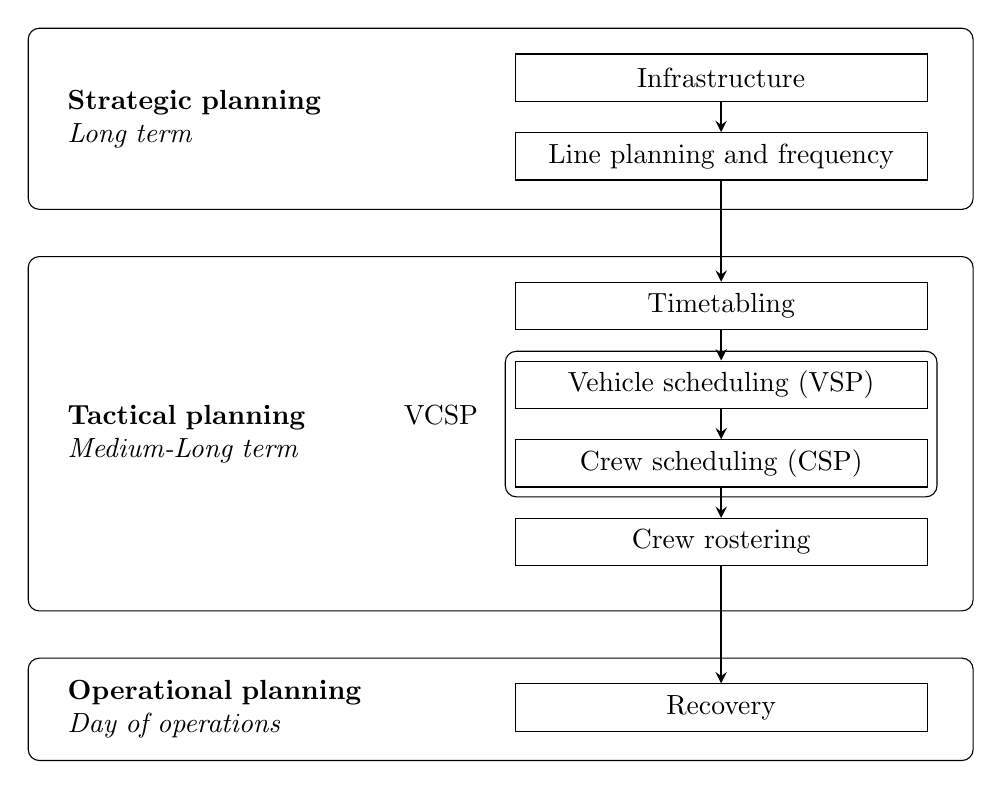
\begin{tikzpicture}[node distance=2cm]
    \node (strategic) [process, minimum height=2.3cm] {\textbf{Strategic planning}\\\textit{Long term}};
    \node at (strategic.base) (infra) [subprocess, xshift=2.8cm, yshift=0.4cm] {Infrastructure};
    \node at (strategic.base) (line) [subprocess, below of=infra, yshift=1cm] {Line planning and frequency};

    \node (tactical) [process, minimum height=4.5cm, below of=strategic, yshift=-2cm] {\textbf{Tactical planning}\\\textit{Medium-Long term}};
    \node at (tactical.base) (timetable) [subprocess, xshift=2.8cm, yshift=1.5cm] {Timetabling};
    \node at (tactical.base) (vehicle) [subprocess, below of=timetable, yshift=1cm] {Vehicle scheduling (VSP)};
    \node at (tactical.base) (crew) [subprocess, below of=vehicle, yshift=1cm] {Crew scheduling (CSP)};
    \node at (tactical.base) (VCSP) [rounded corners, draw=black, fit=(vehicle) (crew), align=left] {\hspace{-4em}VCSP};
    \node at (tactical.base) (rostering) [subprocess, below of=crew, yshift=1cm] {Crew rostering};

    \node (operational) [process, minimum height=1.3cm, below of=tactical, yshift=-1.5cm] {\textbf{Operational planning}\\\textit{Day of operations}};
    \node at (operational.base) (recovery) [subprocess, xshift=2.8cm, yshift=-0.1cm] {Recovery};

    \draw [arrow] (infra) -- (line);
    \draw [arrow] (line) -- (timetable);
    \draw [arrow] (timetable) -- (vehicle);
    \draw [arrow] (vehicle) -- (crew);
    \draw [arrow] (crew) -- (rostering);
    \draw [arrow] (rostering) -- (recovery);
  \end{tikzpicture}
  \caption{A general overview of the public transport planning process, based on \citet{Ceder1986, Ibarra-Rojas2015, Perumal2022LitRev}.}
  \label{fig:planning-overview}
\end{figure}

\subsection{Overview}
The E-VCSP is part of the planning process used in bus public transit, as can be seen in Figure \ref{fig:planning-overview}. It comes directly after the timetabling step, in which \emph{trips} are defined for each line according to passenger demand. Each individual timetabled trip represents a bus traveling along a line at a specified time. Oftentimes, these trips are scheduled regularly throughout the day from the start to the end of a line, however irregular schedules and partial travels along a line are also possible.

With these trips being laid out, we now need to determine how they will be driven. In order to do that, we will create a set of \emph{vehicle tasks}, each representing the schedule for a single vehicle throughout the day. Individual trips often have lengths of around 0.5-2 hours, therefore making it possible to perform multiple trips with a single vehicle and driver in a day. In order to perform a trip, a vehicle must travel to its starting location before driving it; this travel is called a \emph{deadhead}. Deadheads occur between trips and between a trip and a depot, and are generally defined by a driving time and distance between a pair of locations. During a deadhead, the vehicle itself is empty except for the driver. It is therefore beneficial to minimize the total amount of time that vehicles and crew members spend driving deadheads, as costs incurred during this time do not have any direct benefit to passengers.

When considering electric vehicles, the time between trips is not only used for driving deadheads. As electric vehicles generally do not have enough range to drive an entire day, this downtime is also used in order to recharge the vehicle. A variety of different recharging methods are currently in use throughout the industry, however in this work we will exclusively consider conductive charging; specifically, we consider plug-in charging (which is the same method used for most commercial EVs) and pantograph charging. These two techniques share many similarities in their behavior, with the largest difference being the physical connector that is used to connect the power source to the battery. For a detailed overview of available recharging methods and corresponding behavior, we refer the reader to a review by \citet{Zhou2024}.

For conductive charging, recharging stations are often available at the depot, with additional stations sometimes being present at the starting or ending locations of trips (also called the terminal trip stops). Charging stations in the middle of a trip are generally not present. Recharging a vehicle at one of these locations follows a charging curve; this curve defines the charging rate when a vehicle is at a certain state of charge. For the most commonly used battery chemistry, lithium-ion, this curve is generally split into two phases: from 0 to around 80\%, in which the charging rate is roughly constant, and from 80 to 100\%, where it slows significantly. These phases often take similar amounts of time, and depending on the infrastructure available a full charge may take on the order of hours. Fast-charging infrastructure has become more prevalent in recent years with charging speeds of up to $\sim$350km/hour, however this still results in significant time spent charging during a vehicle task.

The resulting vehicle downtime necessitates careful planning of \emph{crew duties}. Crew members must follow local labor regulations, which often consist of maximum driving times throughout the day and required breaks. Combining these breaks with charging time for the vehicle can be beneficial, as this implies that both the crew member and vehicle experience useful idle time. In order to make even better use of paid crew time, crew members may transfer between vehicles throughout the day.

These vehicle \emph{handovers} are often only possible at a predetermined set of locations. These \emph{relief points} have waiting areas or break rooms connected to them, providing a place for a crew member to stay before entering their next vehicle. In order for a handover to take place, a minimum handover time is required, allowing a driver to enter and leave the vehicle. A subset of these relief points may also be used in order to start and end a shift. We shall call these locations \emph{crew bases}; at the start and end of a d. 

As not all location visits are suitable for handovers, a sequence of trips and deadheads which does not visit a relief point (or not for long enough to perform a handover) must be driven by a single driver. Such a sequence is called a \emph{block}, and represents the smallest unit of work that can be performed by a driver. Both vehicle and crew schedules can be seen as a collection of blocks, with possible idle, charging and break times to connect the blocks.

Overall, the goal is to find a set of feasible vehicle tasks and crew duties that minimizes costs. In this, the vehicle tasks must ensure that each trip is driven while minimizing costs incurred by driving and power use. These schedules must also ensure that enough charging takes place such that the vehicle state of charge stays within acceptable levels. Crew schedules, on the other hand, must ensure that each driven block has a driver associated with it without breaking local labor regulations. The goal here is minimizing the overall number of paid hours.

\begin{table}[h]
  \centering
  \begin{tabular}{ll}
    \toprule
    \multicolumn{1}{l}{\textbf{Notation}} & \multicolumn{1}{l}{\textbf{Definition}}               \\
    \cmidrule(lr){1-1}\cmidrule(lr){2-2}
    \multicolumn{2}{l}{\textit{Given}} \\
    $\mathcal{D}$ & The depot \\ 
    $t \in \mathcal{T}$ & Set of all trips, $t$ a single trip \\
    $dh \in \mathcal{DH}$ & Set of all feasible deadheads, $dh$ a single deadhead \\ 
    $b \in B$ & Set of all blocks, $b$ a single block \\
    $vt_i \in VT$ & Set of all vehicle tasks, $vt_i$ single vehicle task \\
    $cd_j \in CD$ & Set of all crew duties, $cd_j$ single crew duty \\
    $d_\chi$ & Amount of charge used driving a trip/deadhead \\
    $u_{l,\sigma,\tau}$ & Max. charge gained at location $dh$ in $\tau$ time with starting SoC $\sigma$ \\
    $\sigma_{start}$ & SoC at beginning of operating period \\
    $\sigma_{min}$ & Minimum SoC of vehicle \\
    $\sigma_{max}$ & Maximum SoC of vehicle \\ 
    \addlinespace[0.6em]
    \multicolumn{2}{l}{\textit{Parameters}} \\
    $k_{i,t}$ & Binary parameter, vehicle task $vt_i$ covers trip $t$ \\ 
    $l_{i,b}$ & Binary parameter, vehicle task $vt_i$ contains block $b$ \\ 
    $m_{j,b}$ & Binary parameter, crew duty $cd_j$ covers block $b$ \\ 
    $d_{j}$ & Parameter, duration of crew duty $cd_j$ \\ 
    $d_{j,\textit{long}}$ & Binary parameter, $d_j > 8.5$ hours \\ 
    $\rho_{j,\chi}$ & Binary parameter, crew duty $cd_j$ is of type $\chi$ \\ 
    \addlinespace[0.6em]
    \multicolumn{2}{l}{\textit{Decision variables}} \\
    $x_{i} \in \{ 0, 1 \}$ & Usage of vehicle task $vt_i$  \\ 
    $y_{j} \in \{ 0, 1 \}$ & Usage of crew duty $cd_j$ \\ 
    \addlinespace[0.6em]
    \multicolumn{2}{l}{\textit{Helper notation}} \\
    $B_\chi \subseteq B$ & Set of blocks in $\chi$ \\ 
    $km(vt)$ & Kilometers traveled during $vt$ \\ 
    $chg(vt)$ & KWh gained during $vt$ \\ 
    $chl(vt)$ & KWh used during $vt$ \\ 
    $br(cd)$ & Total break time in $cd$ \\ 
    $dur(\chi)$ & Total duration of $\chi$ \\ 
    $cost(\chi)$ & Cost of schedule $\chi$ \\ 
    \addlinespace[0.2em]
    \bottomrule
  \end{tabular}
  \caption{Notation used for formal problem description, where $\chi$ is used as a placeholder when multiple argument types can be applied.}
  \label{tab:notation}
\end{table}

\subsection{Formal definition}
We will now formally define the E-VCSP. In this, we consider a variant with a single depot, single vehicle type and charging stations without vehicle capacity limitations. Additionally, partial and non-linear charging are considered. For crew members, we will include a simplified version of the Dutch labor regulations. A summary of the notation used has been provided in Table \ref{tab:notation}.

Let $\mathcal{L}$ be a given set of locations; of these, exactly one location $\mathcal{D} \in \mathcal{L}$ is the depot. Next, a set of trips $\mathcal{T}$ is given based on the timetables of the considered lines; each of these trips starts and ends at a location in $\mathcal{L}$. Let $\mathcal{DH}$ be the set of deadheads that may feasibly be driven; these are provided as pairs of locations within $\mathcal{L}$ with associated distances and driving times, and we will assume that at least the pairs of the form $(l, l)$, $(l, \mathcal{D})$ and $(\mathcal{D}, l)$ exist for all $l\in \mathcal{L}$. Additionally, we will make the assumption that the provided driving times and distances are unaffected by the time of day, and we note that a deadhead may be driven more than once. 

Next, let us define our battery behavior. Let $\sigma_{start}$ represent the SoC of all vehicles in the fleet at the start of the operating period, and let $[\sigma_{min}, \sigma_{max}]$ represent the acceptable SoC operating range for the vehicles. For each trip $t$ and deadhead $dh$, let $d_t$ and $d_{dh}$ respectively indicate the SoC used during the movement. A subset of the locations $\mathcal{L}_c \subseteq \mathcal{L}$ has charging equipment available; for each of these, let $u_{l,\sigma,\tau}$ represent the maximum amount of SoC gained at location $l \in \mathcal{L}_c$ when a vehicle starts at an SoC of $\sigma$ and charges for $\tau$ time; note that this explicitly allows us to model nonlinear charging behavior. 

Lastly, let us define relief points and crew bases. A subset $\mathcal{L}_{rl} \subseteq \mathcal{L}$ of the defined locations may serve as relief points; these locations are the only ones at which a handover or break for a crew member can take place. For each of these locations, a minimum handover time is defined. A subset of these relief points $\mathcal{L}_{cb} \subseteq \mathcal{L}_{rl}$ is a crew base; these locations are the only ones at which a crew member may start or end their duty. For each of these locations, a sign-on and sign-off time are defined in order to get on and off the vehicle at the beginning and end of a shift respectively. 

Let a block be a sequence of trips, deadheads and short idles that must be performed by a single driver; that is, no relief points are visited for long enough to perform a handover during the sequence except at its start and end. Let an individual trip, deadhead or idle in this sequence be called a \emph{block element}. In order for a block to be feasible, it must match the following requirements: 
\begin{itemize}
  \item A block must contain at least one trip or deadhead.
  \item The starting and ending locations of a block are relief points. If additional relief points are visited during the block, the idle time spent there must be less than the minimum handover time.
  \item For any two sequential block elements, the ending location and time of the first element are the same as the starting location and time of the second element.
  \item For each idle time at a charging location $l \in \mathcal{L}_c$ of length $\tau$, a vehicle may charge with some value $\alpha \cdot u_{l,\sigma,\tau}$, where $0 \leq \alpha \leq 1$ represents a fraction of the maximal charge gained. 
  \item There must exist some SoC $\sigma_{start}$ at the beginning of the block, such that the SoC of the vehicle remains within the range $[ \sigma_{min}, \sigma_{max} ]$ throughout the block.
\end{itemize}
Let the set of all feasible blocks be $B$. A schedule for a vehicle throughout the day can now be constructed as a sequence of blocks and idle periods. Let us refer to such a schedule as a \textit{vehicle task}, and let us call the contained blocks and idles \emph{task elements}. In order for a vehicle task to be feasible, the following conditions need to be met:
\begin{itemize}
  \item A vehicle task contains at least one block. 
  \item The starting and ending location of the task are the depot. 
  \item For any two sequential task elements, the ending location and time of the first element are the same as the starting location and time of the second element.
  \item For each idle time at a charging location $l \in \mathcal{L}_c$ of length $\tau$, a vehicle may charge with some value $\alpha \cdot u_{l,\sigma,\tau}$, where $0 \leq \alpha \leq 1$ represents a fraction of the maximal charge gained. 
  \item There must exist some SoC $\sigma_{start}$ at the beginning of the task, such that the SoC of the vehicle remains within $[ \sigma_{min}, \sigma_{max} ]$ throughout the task.
\end{itemize}
Let the set of all feasible vehicle tasks be $VT$. For a vehicle task $vt$, let us define its cost as being $cost(vt) = \gamma_1 + \gamma_2 \cdot km(vt) + \gamma_3 \cdot chg(vt) + \gamma_4 \cdot chl(vt)$, where $km(vt)$, $chg(vt)$ and $chl(vt)$ represent kilometers traveled, charge gained and charge lost during $vt$ respectively and $\gamma$ is a vector of cost scalars.

Next, let us consider crew duties. As with vehicle tasks, a crew duty primarily consists of blocks that need to be driven throughout the day. Crew members are however bound by labor regulations; in most cases, this means that we will need to include break times and a maximum overall duration in the schedule. Additionally, idle time at handover locations may be required in order to wait for an arriving vehicle, and time is spent signing on/off the vehicle at the beginning and end of the day. A \textit{crew duty} therefore consists of a sequence of blocks, idle, break and sign-on/off times. As with blocks and vehicle tasks, we will refer to individual parts of this sequence as \emph{duty elements}. Exact feasibility constraints for crew duties will differ per country and region based on local labor regulations, however in general the following conditions must always be met: 
\begin{itemize}
  \item The crew duty consists of one or more blocks and zero or more break/idle times.
  \item The crew duty must start and end at a crew base; a sign-on at that base must be performed as the first element in the duty, and a sign-off at that base must be performed as the last element of the duty.
  \item For any two sequential duty elements, the ending location and time of the first element are the same as the starting location and time of the second element.
\end{itemize}
In addition to these universal constraints, we also incorporate a simplified version of the Dutch labor regulations into our feasibility. In order to do this we also assume that a duty has a predetermined type; this type defines additional constraints on both the duty itself and the eventual selection of duties that is used in order to cover the required blocks. Let us start by defining the constraints which apply regardless of the duty type:
\begin{itemize}
  \item The crew duty may have a duty length of at most 9 hours. 
  \item A crew duty may contain no span of time longer than 4 hours without a break.
  \item For duties between 4 and 5.5 hours, at least one break of 15 minutes must be included. 
  \item For duties longer than 5.5 hours, at least 40 minutes of break time must be included. All breaks must be longer than 15 minutes, and at least one break must be 20 minutes or longer.
  \item For duties starting after 15:00, at least one break between 16:30 and 20:30 of at least 20 minutes must be included. 
\end{itemize}
In addition to these, the following duty types are defined, each with their own additional constraints:
\begin{itemize}
  \item \textbf{Early} Must end before 16:30.
  \item \textbf{Day} Must end between 16:30 and 18:15.
  \item \textbf{Late} Must start after 13:00 and end before 26:30.
  \item \textbf{Night} Must start before 24:00 and end after 26:30. Duty may be at most 7 hours long.
  \item \textbf{Between} Must start before 13:00 and end after 18:15.
  \item \textbf{Broken} Must start after 5:30 and end before 19:30. The duty is broken in two by a long unpaid idle period of at least 1.5 hours, which starts and ends at a crew base. A sign-off and sign-on must be done in order to perform the long idle. Both parts of the duty are considered individually for the universal break requirements discussed previously.
\end{itemize}
Let the set of all crew duties that match these conditions be $CD$. For a crew duty $cd$ let us define its cost as being $cost(cd) = \beta_1 + \beta_2 \cdot br(c) + \beta_3 \cdot dur(cd) + typ(cd)$, where $br(cd)$ and $dur(cd)$ represent the total break time in and duration of $cd$ respectively, $typ(cd)$ represents a duty type specific cost, and $\beta$ is a vector of cost scalars. 

For a selected set of crew duties $CD' \subset CD$, additional constraints are also in place: 
\begin{itemize}
  \item The average duty length of $CD'$ must be at most 8 hours, excluding time spent in long idles during \textit{broken} duties.
  \item At most 15\% of duties in $CD'$ have a length of more than 8.5 hours.
  \item At most 30\% of duties in $CD'$ are of type \textit{broken}.
  \item At most 10\% of duties in $CD'$ are of type \textit{between}.
\end{itemize} 

\noindent Using all this, we can now formulate a linear program to describe our integrated problem. In this, let $x_i$ and $y_j$ be binary variables indicating the usage of $vt_i \in VT$ and $cd_j \in CD$ respectively. Additionally, let $k_{i,t}$ indicate that $vt_i$ covers trip $t \in \mathcal{T}$, let $l_{i,b}$ indicate that $vt_i$ contains block $b \in B$, and let $m_{j,b} $ indicate that $cd_j$ includes block $b \in B$. Let $\rho_{j,\text{broken}}$ and $\rho_{j,\text{between}}$ indicate whether a duty $cd_j$ is of type \textit{broken} or \textit{between} respectively. In this, $k_{i,t}$, $l_{i,b}$, $m_{j,b}$ and $\rho_{j,\chi}$  are all binary parameters. Lastly, let $d_j$ be a parameter indicating the duration of duty $cd_j$, and let $d_{j,\textit{long}}$ be a binary parameter indicating whether $d_j > 8.5$ hours. Our cost minimization can then be formulated as follows:
\begin{align}
\min \quad
& \sum_{vt_i \in VT} x_{i} \cdot cost(vt_i) + \sum_{cd_j \in CD} y_{j} \cdot cost(cd_j)  
\end{align}
Subject to:
\begin{align}
\sum_{vt_i \in VT} x_{i}k_{i,t} &= 1 && \forall t \in \mathcal{T} \label{form:pd-all-trips-covered} \\
\sum_{vt_i \in VT}x_i l_{i,b} - \sum_{cd_j \in CD}y_j m_{j,b} &= 0 && \forall b \in B \label{form:pd-all-blocks-covered} \\
\sum_{cd_j \in \textit{CD}} y_{j} \cdot (\frac{d_{j}}{\textit{8 hours}} - 1) &\leq 0 && \label{form:pd-max-avg-shift-length}\\
\sum_{cd_j \in \textit{CD}} y_{j} \cdot (0.15 - d_{j,\textit{long}}) &\geq 0 && \label{form:pd-max-long-shifts}\\
\sum_{cd_j \in \textit{CD}} y_{j} \cdot (0.3 - \rho_{j,\textit{broken}}) &\geq 0 && \label{form:pd-max-broken-shifts}\\
\sum_{cd_j \in \textit{CD}} y_{j} \cdot (0.1 - \rho_{j,\textit{between}}) &\geq 0 && \label{form:pd-max-between-shifts}\\
x_{i} &\in \{ 0, 1 \} && \forall vt_i \in VT \\
y_{j} &\in \{ 0, 1 \} && \forall cd_j \in CD
\end{align}
Here, constraint (\ref{form:pd-all-trips-covered}) ensures that all trips are covered by a vehicle, and constraint (\ref{form:pd-all-blocks-covered}) ensures that for each block, the number of assigned drivers is equal to the number of assigned vehicles. Constraint (\ref{form:pd-max-avg-shift-length}) ensures a maximum average duty length, and constraints (\ref{form:pd-max-long-shifts}-\ref{form:pd-max-between-shifts}) ensure that the number of duties which are longer than 8.5 hours / of a certain type are within limits. This integrated formulation minimizes the costs for both vehicle and crew duties simultaneously. For comparison, when the E-VSP and CSP are solved sequentially, the formulation becomes the following. First, vehicle tasks are selected such that their costs are minimized:
\begin{align}
\min \quad
& \sum_{vt_i \in VT} x_{i} \cdot cost(vt_i)
\end{align}
Subject to:
\begin{align}
\sum_{vt_i \in VT} x_{i}k_{i,t} &= 1 && \forall t \in \mathcal{T} \label{form:all-trips-covered-seq} \\
x_{i} &\in \{ 0, 1 \} && \forall vt_i \in VT
\end{align}
Here, constraint (\ref{form:all-trips-covered-seq}) once again ensures that all trips are covered by a vehicle task. Once the vehicle tasks have been selected, we can use them to derive the set of blocks that are driven. Let $B_{vt} \subseteq B$ represent the set of blocks driven by a vehicle task $vt$. The overall set of blocks driven is then $B' = \bigcup_{vt_i \in VT, x_i = 1}B_{vt_i}$, and let the crew duties for which all used blocks appear in $B'$ be $CD'$. Note that in our construction of $B'$, each block is present at most once due to the fact that all trips are covered exactly once in our E-VSP formulation. \\
Using this, our formulation for crew duties becomes the following:
\begin{align}
\min \quad
& \sum_{cd_j \in CD'} y_{j} \cdot cost(cd_j)  
\end{align}
Subject to:
\begin{align}
\sum_{cd_j \in CD'} y_j m_{j,b} &= 1  && \forall b \in B' \label{form:all-blocks-covered-seq} \\
\sum_{cd_j \in CD'} y_{j} \cdot (\frac{d_{j}}{\textit{8 hours}} - 1) &\leq 0 && \\
\sum_{cd_j \in CD'} y_{j} \cdot (0.15 - d_{j,\textit{long}}) &\geq 0 && \\
\sum_{cd_j \in CD'} y_{j} \cdot (0.3 - \rho_{j,\textit{broken}}) &\geq 0 && \\
\sum_{cd_j \in CD'} y_{j} \cdot (0.1 - \rho_{j,\textit{between}}) &\geq 0 && \\
y_{j} &\in \{ 0, 1 \} && \forall cd_j \in CD'
\end{align}
Here, we now consider a greatly reduced number of available blocks and crew duties, resulting in a formulation with significantly fewer rows and columns than the equivalent integrated formulation.

\section{Related work}
In this section, we discuss work related to our research into the E-VCSP. A summary of how batteries and charging behavior are modeled in the discussed works has been included in Table \ref{tab:eVCSP-lit}.

\afterpage{
  \clearpage
  \begin{landscape}
  \null
  \vfill
  \begin{table}[h!]
    \centering
    \begin{tabular}{llllllll}
      \toprule
                                        & Model   & ToU & SoC & Nonlinear Ch. & Partial Ch. & Ch. Location & Degradation \\
      \cmidrule(lr){2-8}
      \citet{Li2014}               & E-VSP   & No  & D   & No            & No          & D            & No          \\
      \Citet{vanKootenNiekerk2017} & E-VSP   & Yes & C/D & Yes           & Yes         & D/T          & Yes         \\
      \citet{Olsen2020}            & E-VSP   & No  & C   & Yes           & Yes         & D/T          & No          \\
      \citet{Zhang2021}            & E-VSP   & No  & C/D & Yes           & Yes         & D            & Yes         \\
      \citet{Parmentier2023}       & E-VSP   & No  & C   & Yes           & Yes         & D/T          & No          \\
      % \citet{Pulyassary2024}       & E-VSP   & No  & C/D & Yes           & Yes         & T            & No          \\
      \Citet{deVos2024}            & E-VSP   & No  & D   & Yes           & Yes         & D/T          & No          \\
      \addlinespace[0.4em]
      \citet{Perumal2021}          & E-VCSP  & No  & C   & No            & No          & D            & No          \\
      \citet{Wang2022}             & E-VCSP  & Yes & C   & No            & Yes         & D            & No          \\
      \citet{Sistig2023}           & E-VCSP  & No  & C   & No            & Yes         & D/T          & No          \\
      \citet{Shen2023}             & E-VCSP  & No  & C   & No            & Yes          & D/T          & No          \\
      \citet{Cong2024}             & E-VCSP  & Yes & C   & No            & Yes         & D            & No          \\
      \addlinespace[0.4em]
      \citet{Ham2021}              & E-VRPTW & Yes & C   & No            & Yes         & D            & No          \\
      \citet{Stadnichuk2024}       & E-TVSP  & No  & C   & No            & Yes         & D/T          & No          \\
      \bottomrule
    \end{tabular}
    \caption{A brief overview of battery modeling in E-VCSP related literature. SoC modeled as (D)iscrete or (C)ontinuous variable, Charge locations at (D)epot or (T)erminal trip stops, Degradation of battery in cost function}
    \label{tab:eVCSP-lit}
  \end{table}
  \vfill
  \end{landscape}
  \clearpage
}

\subsection{(E-)VSP} \label{sec:evsp-litrev}
Before considering previous work on the E-VSP, we first cover the most basic form of vehicle scheduling: that which only considers a single depot, single vehicle type and unlimited vehicle ranges. This problem, often referred to as the Single Depot Vehicle Scheduling Problem (SDVSP), forms the underlying basis of both the multi-depot and electric vehicle extensions that we consider later. We therefore give a brief summary of two common models and solution methods used for the SDVSP, thereby having a baseline to which we can compare extensions. For a more comprehensive overview on different models used for the SDVSP and Multi-Depot VSP (MDVSP), we refer the reader to a review by \citet{Bunte2009}.

In order to find a solution for the SDVSP, the problem can be transformed into one of finding a min-cost flow in a graph. The graph can be constructed as follows: For all trips $\mathcal{T}$, add a pair of nodes representing the start and end of the trip respectively. Add an arc from the start of each trip to its end with capacity 1, lower bound 1 and cost equal to that of driving the trip. Next, connect the end of each trip $t$ to the start of each trip $t'$ for which the deadhead between the two is feasible; that is, there is enough time to drive the deadhead from $t$ to $t'$ before the scheduled starting time of $t'$. Let each of these arcs have a capacity 1 and a cost equal to that of driving the deadhead from $t$ to $t'$. Lastly, let us introduce a pair of nodes representing the depot at the start and end of the day respectively. Connect the depot start node to the start of each trip, and do the same for the depot end node and the end of each trip. For each of these arcs, let the capacity once more be 1 and let the cost be equal to that of driving the deadhead between the depot and trip. Fixed vehicle costs can be represented by adding costs to the arcs leaving the depot.

We can now find the min-cost flow in this graph; in this, let the depot start node be the source, and let the depot end node be the sink. Due to our construction, all trips must be covered by exactly 1 flow, resulting in flow paths which we can directly use as vehicle tasks due to the assumption that our vehicles have infinite range. It is therefore also shown that the SDVSP can be solved in polynomial time, as polynomial time min-cost flow algorithms exist and the graph elements are of size $|V| = O(|\mathcal{T}|)$ and $|A| = O(|\mathcal{T}|^2)$.

Alternatively, the problem can be transformed into one of finding a minimum weight matching within a bipartite graph. The underlying idea is that each trip will have exactly one trip before and after it in a vehicle task, except when it is at the start or end of the task. We can then exploit this by attempting to match trips to their direct successor.

In order to do this, nodes are created for each trip on either side of a bipartite graph, where the left side of the graph represents origins and the right side represents destinations. Additionally, for each available vehicle, a depot node is added on either side of the graph. An edge between an origin-destination pair is added when a feasible deadhead between them exists, and the cost of driving the deadhead is used as its weight. A matching within this graph now represents a collection of vehicle tasks; we can reconstruct a task by starting at a depot node, following its matched edge to the corresponding trip, then using that trip as an origin before repeating until reaching a destination depot. A minimum weight matching within this graph therefore corresponds to a minimum cost set of vehicle tasks which cover all trips.

Two common extensions to the SDVSP make it NP-Hard: the inclusion of multiple vehicle types, as well as the use of multiple depots under the assumption that vehicles must return to their depot of origin. Both of these extensions are also discussed in \citet{Bunte2009}. The modification to the SDVSP flow network is the same in either case: an additional source/sink pair can be added for each new depot or vehicle type, and connected to the trips in the same way as the original depot. The problem then turns into an integral multicommodity flow, which has been shown to be NP-Hard by \citet{Even1975}.

The introduction of any resource constraints within the VSP has also been shown to be NP-Hard (see \citet{Bodin1983}). The E-VSP specifically deals with constraints on the driving range of vehicles, thereby making it closely related to the vehicle scheduling problem with route time constraints (VSP-RTC) as described by \citet{Haghani2002}. The key difference between these two problems is that the E-VSP allows for (partial) recharging of a vehicle throughout the operating period, whereas the VSP-RTC assumes a fixed maximum travel time for the vehicle within the given period. The E-VSP has been shown to be NP-Hard by \citet{Sassi2014}. \\

\citet{Li2014} is one of the first to consider a solution method for the E-VSP. They consider a single-depot case with a single vehicle type, in which the assumption is made that full recharging (or battery swaps) can be performed in a fixed 5-minute time window. The model is based on a modified version of the SDVSP flow network with the inclusion of driving time constraints. Additionally, time-discretized nodes are added to the graph to represent capacitated battery charging/swap stations. Arcs are added from trip nodes to the charging nodes when a travel between the two is feasible, allowing for a vehicle to perform one or more charging action during its task. A variable representing current driving time is updated in each individual node in the graph based on the sum of the driving time of used incoming arcs; by limiting the number of used incoming arcs in a node, charge feasibility is then modeled as an upper bound on each of the driving time variables. Whenever a charging station node is visited, the corresponding variable is reset to 0. As charging nodes are discretized over time, capacity is also enforced using flow-like constraints. 

For smaller instances, this model can be solved to optimality using column generation and branch-and-price (B\&P). For larger instances, an alternate approach using truncated column generation followed by a local search to find a local optimum is used instead. The proposed methods are tested on trips in the San Francisco Bay Area, with a maximum instance size of 242 trips. These tests resulted in optimality gaps of $<5\%$ for buses able to drive 150km, and between 7-15\%  for a range of 120km depending on the instance.

\Citet{vanKootenNiekerk2017} introduce two models which aim to solve the single depot E-VSP while taking into account time dependent energy prices (ToU pricing), nonlinear charging times and battery degradation due to depth of discharge. The first model extends the traditional SDVSP flow model by discretizing the depot nodes over time, and adding a continuous variable to each trip node representing the vehicle SoC at its start. This only allows for the formulation that uses linear charging curves, and does not incorporate degradation or ToU. The second model additionally discretizes both depot and trip nodes for individual starting SoC values. Charge-feasibility of deadheads can then be considered during graph construction, only adding arcs between pairs of nodes when the SoC difference between them can be achieved through driving and charging during the deadhead. This also allows for easy integration of nonlinear charging curves, degradation, and ToU pricing, as the SoC of the vehicle at each discretized trip node is known at construction time. The second model is solved using CG and Lagrangean relaxation. Tests are performed using data provided by Belgian bus company De Lijn in the city Leuven, using a total of 543 trips. They show that the second model can be solved in a considerably shorter time frame for large instances with similar results to the first.

\citet{Olsen2020} consider a multi-depot E-VSP, in which they model the nonlinear phase of charging as an exponential function. In order to solve this problem, they implement a greedy heuristic to construct vehicle tasks. Their primary focus is comparing (piecewise) linear approximations for the second phase of charging with an exponential function based approximation. They conclude that SoC and required charging times are more comparable to real life behavior when using the exponential function.

\citet{Zhang2021} consider an E-VSP variant with a single depot, capacitated charging infrastructure, non-linear charging behavior and battery degradation. They model this by combining elements from \citet{Li2014} and \citet{vanKootenNiekerk2017}, resulting in a network which has time and charge discretized depot, trip and charging station nodes; arcs between these are again only present if the deadhead is both time and charge-feasible. Solutions are found using a combination of CG and B\&P, and tests are performed on both randomly generated instances and 6 not yet electrified lines with up to 160 and 197 trips respectively.

\citet{Parmentier2023} consider a scalable approach to the E-VSP with non-linear charging. They introduce the concept of nondominated charging arcs, which are represented as multiple deadhead arcs between a pair of nodes within the traditional SDVSP network. Their use allows for a number of charging possibilities to be considered between trips when multiple charging points are available, as an arc is only included if there is not another arc available with higher resulting charge and lower cost. In order to solve this problem, a combination of CG and B\&P techniques are used. Testing is done on the \textit{large} instances introduced by \citet{Wen2016} which included up to 8 depots, 16 charging stations and 500 trips. Here, they are able to find solutions that only have an 0.06\% optimality gap.

\Citet{deVos2024} consider the E-VSP with partial recharges and capacitated charging stations. Their model applies a similar discretization as the ones found in the work of \citet{vanKootenNiekerk2017} and \citet{Zhang2021}. As with those models, power used during trips and deadhead arcs is rounded up to the nearest discrete value; this results in an underestimation of the actual SoC of the vehicle during its task, however ensures solutions that can be feasibly driven. This pessimistically rounded graph, which De Vos et al. refer to as the primal network, is accompanied by a dual network; in this graph, power used is rounded down, resulting in more deadheads becoming charge-feasible. Not all paths through this network are feasible vehicle tasks, however the solution cost found using this network is guaranteed to be a lower bound for the solution cost found using the primal network. The problem is solved by applying CG with two separate approaches: branch-and-price and a diving heuristic. In this, the dual network is used in order to generate dual bounds that match those found in a non-discretized model, following ideas presented by \citet{Boland2017}. Testing is performed on a bus concession south of Amsterdam with 816 trips, with subsets being used as smaller instances. Optimality gaps of 1.5-2.7\% are achieved across instances. They additionally note that the framework as provided can easily be extended for nonlinear charging functions and depth-of-discharge battery degradation. 

\subsection{CSP}
Given a solution to the (E-)VSP, the corresponding CSP is most often solved as a set partitioning (or set covering) problem. Here, the tasks described by the sequences of trips generated during vehicle scheduling must be covered by the individual schedules of crew members. This problem has been shown to be NP-Hard in general by \citet{Fischetti1989}.

Research into this subject is primarily done in the context of airline crew planning; crew costs in this field are generally even higher than those found in the more general public transport sector, as shown in \citet{Barnhart2003}. Additionally, strong labor unions and restrictive labor legislation due to safety concerns cause a large number of constraints to be applied to crew schedules, resulting in a non-trivial problem to solve.

Results achieved in the aviation space quite easily generalize to other sectors, and we therefore refer the reader to a review by \citet{Wen2021} for an overview of the state of the art. 

\subsection{(E-)VCSP} \label{sec:evcsp-litrev}
The VCSP is a widely studied problem. Following the call for integrated methods by \citet{Bodin1983} and others in the 1980s, many different methods have been applied to integrate the VSP and CSP. We refer the reader to a recent review by \citet{Ge2024} for a general overview of work done in the field in the past years.

One work that we will individually highlight is that of \citet{Huisman2005}, due to its use of Lagrangean relaxation to connect the VSP and CSP. For readers unfamiliar with the technique, we recommend an introduction by \citet{Beasley1993}. Huisman et al. consider the multi-depot variant, and use a combination of CG and Lagrangean relaxation to solve both the MDVSP and the connection with the CSP. Of note is their assumption that crew members from each individual depot are only allowed to work on trips connected to said depot, allowing for individual depot CSPs to be solved as a subproblem. They test on instances in the Randstad metro area in the Netherlands with a maximum of 653 trips and 4 depots.


As for the electric counterpart of the VCSP, at time of writing we are aware of only five other works that discuss the integrated variant.

\citet{Perumal2021} were the first to offer a solution to the E-VCSP. They consider an instance of the problem in which only full recharges at the depot with a fixed duration of 120 minutes are possible. Solutions are found using ALNS, incorporating a B\&P heuristic for constructing tasks which has been previously used to solve the VCSP, MDVSP and E-VSP by \citet{Haase1996}, \citet{Pepin2009} and
\citet{ vanKootenNiekerk2017} respectively. The authors tested using real life data from lines in Denmark and Sweden with a
maximum instance size of 1109 trips and multiple depots, and report an improvement of $1.17-4.37\%$
across different instances when compared to a sequential approach.

\citet{Wang2022} introduce a two layered model which allows for a mix of traditional combustion and electric buses using Particle Swarm Optimization and an $\epsilon$-constraint based mechanism. The model incorporates partial depot charging, as well as measures to ensure that crew is primarily assigned to the same vehicle throughout the day. A circular bus route with a single depot in Changchun, China with 68 daily trips is used as a basis for testing, with a focus on electric versus diesel usage and driver satisfaction.

\citet{Sistig2023} also offer an ALNS based approach, which aims to incorporate additional flexibility in vehicle scheduling when compared to the work presented by \citet{Perumal2021} by including partial recharges and opportunistic charging at terminal stops of trips. A set ALNS neighborhoods are used in order to solve, where each neighborhood follows a 3-step structure: first a number of improvement rounds is done on the current vehicle solution, then the current crew solution is updated to match the new vehicle solution, before finally doing a number of improvement rounds on the crew solution. The vehicle and crew improvement rounds are themselves also implemented using ALNS algorithms, resulting in nested ALNS rounds being performed. The upper level 3-step neighborhoods only differ in the number of rounds done in each of the two nested ALNS. This approach is tested using an instance of a city route in Germany, with a single depot and a total of 282 trips. Different scenarios based on possible crew break and relief locations were considered in order to compare diesel and electric TCO. Additionally, sensitivity analysis of the TCO was done for parameters such as costs for electricity and drivers.

\citet{Shen2023} provide a minimum-cost flow based framework for the E-VCSP. They consider the single depot variant, in which partial recharges are possible. Solutions are found by first generating a subset of all feasible blocks and corresponding crew duties using a matching-based heuristic approach. Afterwards, a MIP formulation is used to select crew duties and create corresponding vehicle tasks that cover all trips. A city line in China with 270 daily trips and a single depot is used for testing, resulting in cost savings of up to 8.7\% when compared to a sequential approach.

\citet{Cong2024} take a hybrid MIP and SAA based approach to optimize a mixed fleet of combustion and electric vehicles with ToU electricity pricing. In each SAA iteration, a collection of new E-VSP trip assignments are created using neighborhood operations, after which two MIP models are sequentially employed to solve for charging and crew schedules. The methods are tested on a collection of 3 bus routes originating from the same depot in Changchun City, China with a total of 520 trips across all routes. When compared to the sequential approach, the integrated vehicle schedule was able to reduce costs by 0.8\%. 

\subsection{Other related fields}
The VSP is closely related to the vehicle routing problem (VRP); in this problem, the aim is to find minimum cost routes for vehicles originating from a depot that need to pass multiple stops, most commonly for pickup or delivery with capacity constraints. The extension of the E-VRP which includes arrival time windows (E-VRPTW) is most closely related to the E-VSP, as the use of 0-width windows allows us to define the same precedence constraints as those naturally defined by trips in the VSP.

An example of work done on the E-VRPTW is that of \citet{Ham2021}. They consider a single depot case in which they model ToU pricing and partial recharges during delivery routes. In order to model costs, a lexicographical minimization is done over the number of vehicles used, total distance traveled and energy recharged. In order to solve, a hybrid MIP and CP algorithm is used in which CP is used to model ToU related variables, and MIP is used to model the rest of the constraints.

Research has also been done into integrating the E-VSP with the step before it in the planning sequence: timetable planning. This problem, the E-TVSP, has recently been studied in the work of \citet{Stadnichuk2024}. They allowed results of the E-VSP to introduce optimality cuts into the MIP used for creating timetable plans, thereby reducing overall cost. This is achieved by transforming the E-VSP problem into one of bin packing with conflicts, after which three different heuristic methods are applied and compared. They additionally prove that the bounds of the used heuristics are tight for their given instances. 

\subsection{Research gap}
As can be seen in Table \ref{tab:eVCSP-lit}, research into the E-VSP has successfully incorporated many battery characteristics which can be of importance when determining overall operational costs and feasibility. The E-VCSP on the other hand has seen less progress: both non-linear charging and battery degradation have not yet been considered in any work at the time of writing. Additionally, no documented attempt at using a discretized SoC model for the E-VCSP has been made. In this work, we aim to address one of these points: incorporating non-linear charging curves. 

\section{Methodology}
In this section, we will discuss our methodology for solving the E-VCSP. In order to do so, we will first discuss our ways of solving the E-VSP and CSP sequentially; afterwards, we discuss how parts of these techniques can be reused in order to solve the integrated problem.

For both the E-VSP and CSP, a column generation approach is implemented based on a set cover ILP. In order to make this approach computationally feasible, a combination of pre- and postprocessing is applied on the underlying networks and solutions. As large parts of the solution methods for these two problems are shared, a detailed overview of any shared technique will only be provided in the E-VSP section. Where applicable, the CSP solution method will refer back to this. 

For the E-VCSP, a column generation approach in combination with a number of heuristics is once again employed in order to improve upon a solution found by using the sequential methods. As we reuse parts of the sequential approach, we will again refer back to previous sections where possible.

\subsection{E-VSP} \label{sec:evsp-methodology}
Our approach for solving the E-VSP can roughly be broken up into 3 steps: 
\begin{itemize}
  \item \textit{Preprocessing}, in which our initial data set is transformed into a graph which is simplified using heuristics.
  \item \textit{Solving}, in which column generation using various sources is applied in order to solve the problem of finding a set of vehicle tasks which cover all trips. 
  \item \textit{Postprocessing}, in which duplicate trips are transformed into deadheads in order to reduce the total number of driving hours required. 
\end{itemize} 
\subsubsection{Preprocessing}
Given are a set of trips $\mathcal{T}$, a set of locations $\mathcal{L}$, and a set of possible deadheads $\mathcal{DH}$ connecting pairs of locations. Exactly one location $\mathcal{D} \in \mathcal{L}$ is the depot. Additionally, a subset of the locations $\mathcal{L}_c \subseteq \mathcal{L}$ has charging equipment installed. In order to keep notation compact, let us use $s(t)$ and $e(t)$ to refer to the start and end time of a trip $t \in \mathcal{T}$; let us also use $o(t)$ and $d(t)$ to refer to the origin and destination location of $t$.

We now transform this data into a graph $G_{vt} = (V_{vt}, A_{vt})$. Let $V_{vt} = \{ d_{s}, d_{e} \} \cup \mathcal{T}$, where $d_{s}$ and $d_{e}$ represent the depot at the beginning and end of the day respectively. For each node $t \in \mathcal{T}$, add an arc to $A_{vt}$ from $d_{s}$ to $t$ and from $t$ to $d_{e}$ if there is a deadhead in $\mathcal{DH}$ connecting the depot to $o(t)$ and $d(t)$ respectively. Next, add an arc to $A_{vt}$ between each pair of trips $t, t'$ if there is a deadhead in $dh \in \mathcal{DH}$ that connects the $d(t)$ to $o(t')$ and the duration of $dh$ does not exceed $s(t') - e(t)$. This graph corresponds roughly to the one found in the standard VSP formulation as described in Section \ref{sec:evsp-litrev}. Before giving a visualization, we will first modify it slightly in order to be more computationally efficient and include to additional charging capabilities.

Let us begin by reducing the overall size of the graph. In order to do this, let us first consider a single line within the provided timetable. Throughout the day, the number of trips traveling in one direction along the line will be roughly equal to the number of trips traveling the other direction. When this is the case, planned trips are often staggered such that a bus arriving at one end of the line can directly be used in order to drive to the other end, minimizing the amount of vehicle downtime. When considering the timetable as a whole, this pattern may also be found when combining multiple lines: a vehicle arriving after driving a trip on line A may be perfectly timed in order to then drive a trip on line B, assuming A and B share an endpoint. As these connections are often very good to include in a vehicle task due to short idle times, a timetable which contains these patterns can be used to substantially reduce the number of arcs in the graph by forcing the use of these short turnarounds. 

More formally: for each trip node $t$, let $A_t \subset A_{vt}$ be the set of all outgoing arcs from $t$ to other trip nodes. Let $A_{t,st} \subseteq A_t$ be the collection of arcs in which for each arc from $t$ to $t'$ in $A_{t,st}$, $d(t) = o(t')$ and $s(t') - e(t) \leq \delta$ for some threshold $\delta$. If $|A_{t,st}| \geq 1$, replace $A_t$ with $A_{t,st}$ in $A_{vt}$. Otherwise, leave the original set of outgoing arcs the same. A $\delta$ in the order of $0$ to $0.5$ hours was found to be reasonable during initial testing, providing a balance between the number of arcs in the graph and the solution quality.

Once this initial reduction of arcs between trips has been performed, we will extend the remaining arcs in order to better accommodate charging. Let us first assume that charging never occurs when driving to or from the depot; all charging operations will therefore take place in the time between pairs of trips. Additionally, let us assume that whenever we are idle at a charging station, we will charge. Given the current state of our graph $G_{vt}$, this implies that charging exclusively takes place if a trip starts or ends at a charging location, and a connecting trip allows for more idle time than the minimum charging time. Depending on the trips provided, this might not be sufficient to make a good set of vehicle tasks as there is no guarantee that $d(t)$ or $o(t)$ are in $\mathcal{L}_c$.

Let us therefore increase the number of available charging options by considering the existing arcs in $A_{vt}$ between pairs of trips $t$ and $t'$; let us refer to these arcs as \emph{base arcs}. For each charging location $l_c \in \mathcal{L}_c$ for which $l_c \neq d(t)$ and $l_c \neq o(t')$, we will attempt to add another charging arc. This arc will model the possibility of performing a detour between $t$ and $t'$ to $l_c$ in order to charge there; let us refer to one of these arcs as a \emph{detour arc}. Let us add a detour arc if there exists a deadhead $dh \in \mathcal{DH}$ from the $d(t)$ to $l_c$, a deadhead $dh' \in \mathcal{DH}$ from $l_c$ to $o(t')$, and the combined duration of $dh$ and $dh'$ allows for enough time at $l_c$ to meet the minimum charging time. 

With this, we have completed all modifications required in order to solve the E-VSP. An example graph $G_{vt}$ after all modifications have been completed is shown in Figure \ref{fig:evsp-graph}.

\begin{figure}[h]
  \centering
  \begin{tikzpicture}[
    node distance=25mm and 18mm,
  ]
  % Nodes
  \node[circle, draw=black] (ds) {$d_s$};
  \node[lsnode, right=8mm of ds, yshift=16mm] (t1) {Trip 1};
  \node[lsnode, right=20mm of ds, yshift=-10mm] (t2) {Trip 2};
  \node[lsnode, right=8mm of t1, yshift=-8mm] (t3) {Trip 3};
  \node[lsnode, right=12mm of t3, yshift=-8mm] (t4) {Trip 4};
  \node[circle, draw=black, right=15mm of t4] (de) {$d_e$};

  % Outgoing ds
  \draw[->] (ds.south east) -- (t2.west);
  \draw[->] (ds.north east) -- (t1.west);
  \draw[-] (ds.east) -- (t3.west);
  \draw[->] (ds.east) -- (t4.west);

  % Outgoing t1
  \draw[-] (t1.east) -- (t3.west);
  \draw[-, rounded corners] ($(t1.east) + (0,2mm)$) -- ($(t3.east) + (-1mm,5mm)$) -- (de.north west);

  % Outgoing t2
  \draw[-, rounded corners] (t2.east) -- ($(t4.west)+(0,-2mm)$);
  \draw[->, dashed, rounded corners] (t2.east) -- ($(t2.east)!0.5!(t4.west) + (0,1.5mm)$) -- ($(t4.west)+(0,-2mm)$);
  \draw[->, rounded corners] (t2.east) --($(t4.east) + (-1mm,-5mm)$) -- (de.south west);

  % Incoming / outgoing t3 
  \draw[->] ($(t3.west) + (-0.01mm,0.004mm)$) -- (t3.west);
  \draw[->] ($(t3.east) + (0,-2mm)$) -- ($(t4.west) + (0,2mm)$);
  \draw[->, rounded corners] (t3.east) -- ($(t4.east) + (-1mm,5mm)$) -- (de.north west);

  % Outgoing t4
  \draw[->] (t4.east) -- (de.west);

  % Time
  \draw[->] ($(ds) + (0,-22mm)$) -- ($(de) + (0,-22mm)$);
  \node at ($(ds) !0.5! (de) + (0,-19mm)$) {Time};
  \end{tikzpicture}
  \caption{Example of $G_{vt}$ with 4 trips. A possible outgoing arc from Trip 1 to Trip 4 has been removed, as $s(t_3) - e(t_1) \leq \delta$. Between Trip 2 and Trip 4 a dashed detour arc is included.}
  \label{fig:evsp-graph}
\end{figure}

For all detour arcs, we assume that the time at the charging location is maximized. This means that we always perform the deadhead towards the charging location at the earliest possible time, and the deadhead to the next trip at the latest possible time. For base arcs, let us also uniquely define where we will spend our idle time by maximizing time at a charging location if one is present. If no charging location is present, instead attempt to maximize time spent at a relief location. If no relief locations are present or a tie occurs, maximize time spent at the starting location. 

For both types of arcs, we have now uniquely defined the sequence of deadheads and idles which take place before performing the next trip; as this trip is already known, let us include it into our arc as well. Each arc between trips in $A_{vt}$ can therefore be defined as containing 1 or 2 deadheads, a (charging) idle and a trip. Using this, the cost of an arc can be defined as the driving cost of all movements plus the KWh cost of the energy used during the arc. As a consequence of this formulation, we note that each trip node $t \in V_{vt}$ represents the point in time directly following its corresponding trip; nodes do not have an associated cost, as this is already included in the arcs. 

Any feasible vehicle task can now be described as a path in $G$ from $d_s$ to $d_e$. The costs for a task can be defined as a base cost of using a vehicle plus the sum of all used arc costs. In this, we make the assumption that the cost of energy remains constant throughout the day and at different charging locations, and that vehicles will be fully recharged overnight for the same KWh cost as during the day. Additionally, note that not every path from $d_s$ to $d_e$ describes a feasible vehicle task; depending on the arcs used, the amount of time that a vehicle has to charge may not be sufficient in order to keep it within SoC bounds during the task. As we previously defined how much time is spent at a charging location during an arc, this information can be used to determine whether a given path through the graph is a feasible task or not.

\subsubsection{Solving}
In order to now solve the E-VSP, a collection of feasible vehicle tasks that cover the trips $\mathcal{T}$ must be found. In order to do this, we use a column generation approach; this has previously been shown to be an effective solution method for the E-VSP by works such as \citet{vanKootenNiekerk2017}, \citet{Zhang2021} and \citet{deVos2024}. The ILP used to model this is based on a set covering formulation. In this let $VT$ represent the available set of vehicle tasks, let $x_{i}$ be a binary decision variable indicating the use of vehicle task $vt_i \in VT$, and let $k_{i,t}$ be a parameter defining whether vehicle task $vt_i$ includes the trip $t \in \mathcal{T}$.
\begin{align}
\min \quad
& \sum_{vt_i \in VT} x_{i} \cdot cost(vt_i)
\end{align}
Subject to:
\begin{align}
\sum_{vt_i \in VT} x_{i}k_{i,t} &\geq 1 && \forall t \in \mathcal{T} \label{form:vehicle-cover}\\
x_{i} &\in \{ 0, 1 \} && \forall vt_i \in VT \label{form:x-integer}
\end{align}
Here, constraint (\ref{form:vehicle-cover}) ensures that all trips are covered by at least one vehicle task. We note that we allow overcoverage of trips in this formulation in order to increase the feasible solution space; in the event that trips are driven multiple times in a final solution, we will resolve this using postprocessing as described in Section \ref{sec:evsp-postprocessing}.

This ILP can be relaxed to an LP by replacing constraint (\ref{form:x-integer}) with the following:
\begin{align}
x_{i} &\geq 0 && \forall vt_i \in VT
\end{align}
In this relaxed problem, let the dual cost of constraint (\ref{form:vehicle-cover}) be $\pi_t$ with $t \in \mathcal{T}$. For a new vehicle task $vt_0$, its reduced cost would become the following:
\begin{align}
& \text{cost}(vt_0) - \sum_{t \in \mathcal{T}} k_{0,t} \pi_{t} 
\end{align}
Or put simply: the base cost of driving the task minus the sum of the dual costs of the covered trips.

In order to find an initial solution, a local search algorithm is used; this attempts to generate a set of vehicle tasks that covers all trips exactly once with minimum cost. This local search can be run multiple times, after which all generated columns are provided as $VT$ to the LP relaxation, allowing a good base solution to be found. Then, two methods are proposed in order to generate new useful columns by solving the pricing problem: a labeling algorithm and another local search. We will go into more details on all 3 mentioned techniques in the next sections. 

Columns are generated in rounds until no new vehicle tasks with negative reduced costs can be found, or until a predetermined time limit is reached. In each of these rounds, a column generation method is selected, and the current dual costs $\pi$ are used in order to solve the pricing problem. Once no more improvement can be found or the time limit is reached, the constraint (\ref{form:x-integer}) is reinstated, making the model binary again. As early termination is included, this approach can be seen as a form of truncated column generation. In order to then solve our original ILP, branch-and-bound is applied in order to find an integer solution with the columns that were generated up until that point.

\paragraph{Initial solution - Local search} \label{sec:evsp-initial-local-search}
In order to find a good set of initial vehicle tasks, a local search is applied inspired by \citet{Bosch21}. More specifically, a simulated annealing algorithm is used in which an initial set of vehicle tasks is continually modified with the hope of finding a lower cost coverage for our trips. For more details on the workings of a simulated annealing algorithm we refer to \citet{Kirk83}, however a simplified outline has been provided in Algorithm \ref{alg:evsp-simulated-annealing} for readers unfamiliar with the technique.

\begin{algorithm}
\caption{Generic Simulated Annealing}\label{alg:evsp-simulated-annealing}
\begin{algorithmic}
\State $sol \gets InitialSolution()$
\While{$currIt < totalIts$} 
    \State $op \gets operations.GetRandom()$
    \State $sol' \gets op(sol)$
    \If{$\exp((sol.Cost - sol'.Cost) / T) > \textit{uniform}(0, 1)$}
      $sol \gets sol'$
    \EndIf
    \State $T \gets T * \alpha;\:currIts \gets currIts + 1$
\EndWhile
\end{algorithmic}
\end{algorithm}

We initialize our set of covering vehicle tasks by introducing exactly one task for each trip. Then, we will continually try to improve this set by recombining (parts of) the tasks with each other, always accepting a change if it results in better costs and accepting it with a chance proportional to the increase in costs otherwise. In order to make the modification of tasks during this process easier, it is beneficial to include the arcs previously discarded in our short turnaround preprocessing step. By doing this, an intermediate solution of the local search may contain a large vehicle idle time which can be filled by a future operation. In order to further enlarge the solution space, the SoC of the vehicle is allowed to go below the provided minimum SoC of $\sigma_{min}$; a penalty is applied both for the number of times that the vehicle goes below this threshold and the total SoC deficit. During the search, this penalty is progressively increased in order to discourage SoC infeasibilities in the final solution. Both of these methods are also applied to the local search that we will discuss in Section \ref{sec:evsp-pricing-local-search}.

The following set of operations is used in order to modify the set of vehicle tasks. Of these, the first two are almost directly taken from \citet{Bosch21}, with the addition of support for detour arcs between pairs of trips. The last operation is added in order to handle switching between base and detour arcs, as in our instances trips may not always pass the charging locations frequently enough in order to charge throughout the day. During the algorithm, the operations are chosen at random from a weighted distribution.

\noindent\subparagraph{2-Opt (or tail swap)}  Two different vehicle tasks $vt$ and $vt'$ are selected at random from the available set of tasks. Next, a time $t$ is randomly selected such that $t$ does not fall inside a trip in either $vt$ or $vt'$. All trips after $t$ in $vt$ are moved to $vt'$, while at the same time moving all trips after $t$ in $vt'$ to $vt$. In order to connect the tails to the parts of the tasks before $t$, a random arc between the preceding depot / trip and the start of the tail is selected from $A_{vt}$. If the schedule resulting cannot be made as there are no arcs available to reconnect the tails, the swap is reverted. If either $vt$ or $vt'$ becomes empty due to the entirety of its schedule being swapped to the other task, remove the empty task from the available set. A visual representation of this operation is shown in Figure \ref{fig:2opt-vt}.
\begin{figure}[H]
  \centering
  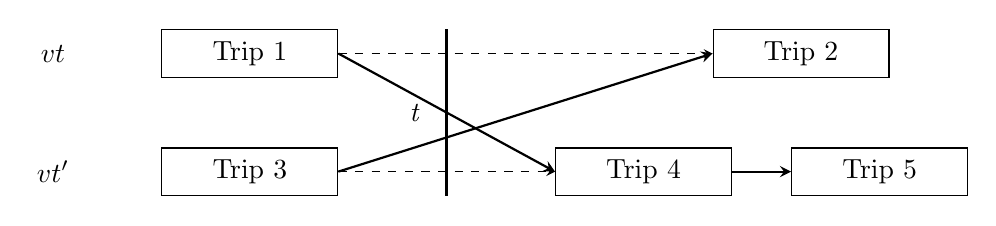
\begin{tikzpicture}[node distance=2cm]
    \node (vt1) [xshift=-2.5cm] {$vt$};
    \node (vt2) [xshift=-2.5cm, yshift=-1.5cm] {$vt'$};
    
    \node (t1) [lsnode] {Trip 1};
    \node (t2) [lsnode, xshift=7cm] {Trip 2};

    \node (t3) [lsnode, yshift=-1.5cm] {Trip 3};
    \node (t4) [lsnode, yshift=-1.5cm, xshift=5cm] {Trip 4};
    \node (t5) [lsnode, yshift=-1.5cm, xshift=8cm] {Trip 5};

    % Original arcs
    \draw [dashedarrow] (t1) -- (t2);
    \draw [dashedarrow] (t3) -- (t4);
    \draw [arrow] (t4) -- (t5);

    % New arcs
    \draw [arrow] (t1.east) -- (t4.west);
    \draw [arrow] (t3.east) -- (t2.west);

    % Thick vertical bar between t3 and t4
    \coordinate (barTop) at ($(t3.north)!0.5!(t4.north) + (0,1.5cm)$);
    \coordinate (barBot) at ($(t3.south)!0.5!(t4.south)$);
    \draw[very thick] (barTop) -- (barBot);

    % Label "t" to the left of the bar, vertically centered
    \node[] at ($(barTop)!0.5!(barBot) + (-0.4cm,0)$) {\textit{t}};
  \end{tikzpicture}
  \caption{2-Opt operation on two vehicle tasks $vt$ and $vt'$. Trips after $t$ (2 for $vt$, 4 and 5 for $vt'$) are moved to the other task. Arrows are arcs in $A_{vt}$, dashed arrows between trips are replaced by solid arrows during operation.}
  \label{fig:2opt-vt}
\end{figure}
\noindent\subparagraph{Range move} Two different vehicle tasks $vt$ and $vt'$ are selected at random from the available set of tasks. Next, from $vt'$, a random continuous range of trips $r$ is selected; $r$ is removed from $vt'$ and is added to $vt$. In order to connect $r$ to preceding and following nodes in $vt$, random arcs within $A_{vt}$ are chosen. The same is done in order to reconnect the remainder of $vt'$. As before, if the resulting vehicle tasks cannot be made due to arcs missing in $A_{vt}$, the change is reverted. If $vt'$ becomes empty due to the removal of $r$ and the change is accepted, remove $vt'$ from the available set of vehicle tasks. A visual representation of this operation is shown in Figure \ref{fig:rangemove-vt}.
\begin{figure}[H]
  \centering
  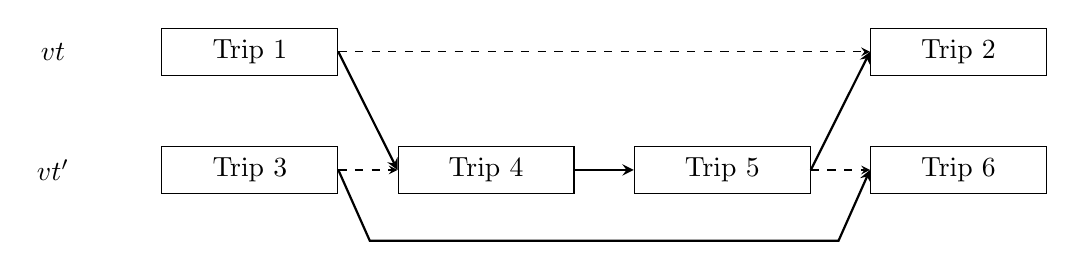
\begin{tikzpicture}[node distance=2cm]
    \node (vt1) [xshift=-2.5cm] {$vt$};
    \node (vt2) [xshift=-2.5cm, yshift=-1.5cm] {$vt'$};

    \node (t1) [lsnode] {Trip 1};
    \node (t2) [lsnode, xshift=9cm] {Trip 2};

    \node (t3) [lsnode, yshift=-1.5cm] {Trip 3};
    \node (t4) [lsnode, yshift=-1.5cm, xshift=3cm] {Trip 4};
    \node (t5) [lsnode, yshift=-1.5cm, xshift=6cm] {Trip 5};
    \node (t6) [lsnode, yshift=-1.5cm, xshift=9cm] {Trip 6};

    % Original arcs
    \draw [dashedarrow] (t1) -- (t2);
    \draw [dashedarrow] (t3) -- (t4);
    \draw [arrow] (t4) -- (t5);
    \draw [dashedarrow] (t5) -- (t6);

    % New arcs after move
    \draw [arrow] (t1.east) -- (t4.west);
    \draw [arrow] (t5.east) -- (t2.west);

    \draw [arrow] (t3.east) -- ++(0.4,-0.9) -- ($(t4)!0.5!(t5)+(0,-0.9)$) -- ($(t6.west)+(-0.4,-0.9)$) -- (t6.west);
  \end{tikzpicture}
  \caption{Range move operation on two vehicle tasks $vt$ and $vt'$. A continuous range of trips (here, trips 4 and 5) are moved from $vt'$ to $vt$.}
  \label{fig:rangemove-vt}
\end{figure}

\noindent\subparagraph{Change arc} A single vehicle task $vt$ is selected at random from the available set of tasks. In this task, an arc $a$ connecting two trips is selected for which there exist alternative connecting arcs in $A_{vt}$. One of these alternative arcs is selected at random in order to replace $a$. As not all base arcs allow for charging, this operator can allow for a new charging opportunity to be added to a task; this in turn may result the reduction of penalties or for more trips to be added later. On the other hand, if a detour arc is currently selected without it being required to keep the vehicle SoC within bounds, it may be removed to save on driving costs. A visual representation of this operation is shown in Figure \ref{fig:changearc-vt}.
\begin{figure}[h]
  \centering
  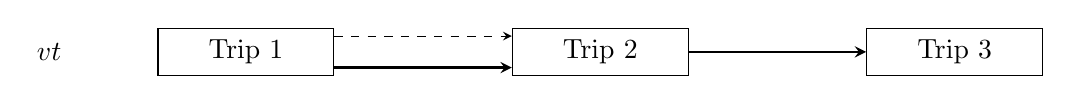
\begin{tikzpicture}[node distance=2cm]
    \node (vt1) [xshift=-2.5cm] {$vt$};

    \node (t1) [lsnode] {Trip 1};
    \node (t2) [lsnode, xshift=4.5cm] {Trip 2};
    \node (t3) [lsnode, xshift=9cm] {Trip 3};

    % Original arcs
    \draw [dashedarrow] ($(t1.east) + (0, 0.2cm)$) -- ($(t2.west) + (0, 0.2cm)$);
    \draw [arrow] (t2) -- (t3);

    % new arc
    \draw [arrow] ($(t1.east) + (0, -0.2cm)$) -- ($(t2.west) + (0, -0.2cm)$);
  \end{tikzpicture}
  \caption{Change arc operation on vehicle task $vt$. The arc between trip 1 and trip 2 is replaced by a different arc in $A_{vt}$, changing the SoC of the vehicle when entering trip 2.}
  \label{fig:changearc-vt}
\end{figure}

\noindent Once all iterations have been completed, some vehicle tasks may still contain SoC infeasibilities. If this is the case, a number of additional iterations are performed on the tasks with infeasibilities with only the \textit{Change arc} operator. If this is not able to fix the SoC infeasibilities, the task is discarded and each for each trip in the task, a task with only that trip is added to the solution instead.

As the operations are randomly chosen, the resulting vehicle tasks (and corresponding quality) might differ greatly between two different runs. We therefore run the algorithm a number of times, thereafter allowing the LP relaxation to use the best available combination of columns in order to find an initial cover for the trips. 

\paragraph{Pricing problem - Labeling} \label{sec:labeling-evsp}
Let us consider our previously defined graph $G_{vt} = (V_{vt}, A_{vt})$. In order to solve the pricing problem, let us slightly modify the costs of the arcs within our graph such that finding a path of minimum cost from $d_s$ to $d_e$ corresponds to a path of minimum reduced costs. In order to do this, for each trip $t$, let us subtract the reduced cost $\pi_t$ from the costs of each incoming arc. Now, the sum of arc costs for any path from $d_s$ to $d_e$ corresponds to the reduced costs of that path, transforming our pricing problem into a search for a shortest feasible path from $d_e$ to $d_s$.

As we have to keep our SoC within bounds, this problem is a variant of a resource-constrained shortest path problem. In order to solve this, we apply a labeling algorithm, inspired by \citet{Huang2016}. Here, starting from a source, we will propagate an achievable state (or label) through each outgoing arc; then, we select a new label and do the same, continuing until all labels can no longer be propagated further. A sketch of a generic labeling algorithm is outlined in Algorithm \ref{alg:evsp-labeling}. In our case, for each node in $\{ d_s \} \cup T$, we keep track of a set of active labels. Each of these labels contains the current costs and current SoC; the previous label may also be stored in order to make backtracking easier. Starting in $d_e$ with an empty label, we will propagate labels through the graph. In this, let us refer to the collection of labels that reach a certain node as being \textit{contained} in that node. 

\begin{algorithm}
\caption{Generic Labeling}\label{alg:evsp-labeling}
\begin{algorithmic}
\State $activeLabels.Init()$ \Comment{List of node / label pairs}
\State $allLabels.Init()$ \Comment{Map from node to list of labels}
\While{$|\textit{activeLabels}| > 0$} 
    \State $(label, node) \gets \textit{activeLabels.Pop()}$
    \For{$arc \in node.OutgoingArcs$}
        \State $(label', node') \gets ApplyArc(label, arc)$
        \If{$Infeasible(label')$} 
          \textbf{continue}
        \EndIf
        \State $allLabels[node'].Push(label')$
        \If{$node' \neq endNode$}
          \State $activeLabels.Push(label', node')$
        \EndIf
    \EndFor
\EndWhile
\end{algorithmic}
\end{algorithm}
Once all active labels have been processed, $d_e$ will now contain a list of finalized labels. We can then find the label with the lowest costs and backtrack through previous labels to $d_s$ in order to reconstruct the entire vehicle task. If the reduced cost of this task is negative, it will improve our solution to the relaxed E-VSP when included. 

As the number of outgoing arcs may be large, propagating all labels can become computationally expensive. We therefore implement a domination rule used by \citet{Huang2016}, allowing us to discard a label if a better one is known: for two labels $l$ and $l'$ in the same node $v$, we consider $l$ to be dominated by $l'$ if the costs of $l'$ are not higher and the SoC of $l'$ is not lower. If a label $l$ is dominated after the introduction of a new label $l'$ in $v$, the label $l$ is removed from the list of active labels, reducing the total number that need to be considered for propagation.

In order to make this domination rule stronger, SoC values are binned into discrete buckets. This allows for small SoC differences to be disregarded when checking for domination, allowing more labels to become dominated and further reducing computational load. During our testing, actual SoC values were rounded down to the nearest whole percentage point for domination purposes, resulting in a total of 101 buckets. Major gains can also be achieved through proper processing order of active labels. As $G_{vt}$ is a DAG due to arcs going forward in time, a topological sorting of the nodes can be constructed. If active labels are then evaluated in this order, it is guaranteed that all domination rulings for a certain trip node will have been applied before any labels of that node are expanded. This greatly reduces the total number of labels expanded, reducing overall runtime.

The list of finalized labels in $d_e$ often contains more than one label with negative costs; in this case, multiple vehicle tasks with negative reduced costs can be extracted from the labeling result. In order to do this, we first sort the labels by cost in non-descending order. A maximum of $N_{\textit{VT,LB}}$ labels is then selected from this sorted list. In order to encourage good coverage of all trips within a single column generation round, an attempt is first made to select labels whose trip covers are disjoint. After no more labels are available whose cover is disjoint from those already selected, we simply add labels with new trip covers until we have added $N_{\textit{VT,LB}}$ in total or until all labels with unique trip covers and negative reduced costs have been added. 

While this allows us to converge on a good solution for the relaxed problem quite quickly, solving the ILP with the resulting vehicle tasks might still prove challenging without significant trip overlap. In an attempt to prevent this, a secondary set of vehicle tasks is generated, inspired by \cite{Guido2009}. In this, the top $M_{\textit{VT,LB}} \leq N_{\textit{VT,LB}}$ generated tasks from the initial labeling round are selected as a base. For each of these bases, we iteratively block off some of the trips from the task, starting from the front. For each set of blocked off nodes, we then rerun the labeling algorithm; this causes a new set of labels to be generated which might still use part of the base, but are forced to use alternate trips for the parts which are blocked off. This results in vehicle tasks with new covers which might not be optimal in the relaxation, however they might help during the final solve.

\paragraph{Pricing problem - Local search} \label{sec:evsp-pricing-local-search}
Without binning of SoC values, the labeling algorithm provides an exact solution to the pricing problem. For larger instances however, it might not be computationally feasible to generate enough columns in order to find a good solution. As an alternative, we can approximate a solution to the pricing problem by once again using a simulated annealing algorithm. Here, we now attempt to construct a single vehicle task with minimum reduced costs. As previously discussed in Section \ref{sec:evsp-initial-local-search}, it can be beneficial to increase the number of feasible intermediate solutions by not applying filtering of arcs in $A_{vt}$ during preprocessing and using penalties for SoC infeasibilities.

Starting with an empty task $vt$, a collection of operations is again repeatedly applied in order to modify it. After an operation has been applied, the reduced cost of the new vehicle task is compared to that before the change in order to check for acceptance. The following set of operations is used in order to construct our vehicle task: 

\subparagraph{Add trip} From the set of currently unvisited trips, select a trip $t$ at random. Let $t_{pred}$ and $t_{succ}$ be the latest trip before $t$ and earliest trip after $t$ currently in $vt$ respectively. If $t_{pred}$ is defined, select a random arc from $t_{pred}$ to $t$ from $A_{vt}$ in order to connect $t$ into $vt$. Do the same for $t$ and $t_{succ}$. If the resulting task is infeasible (either through scheduling conflicts or no connecting arcs existing), the change is rejected. A visual representation of this operation is shown in Figure \ref{fig:addtrip-vt}.

\begin{figure}[h]
  \centering
  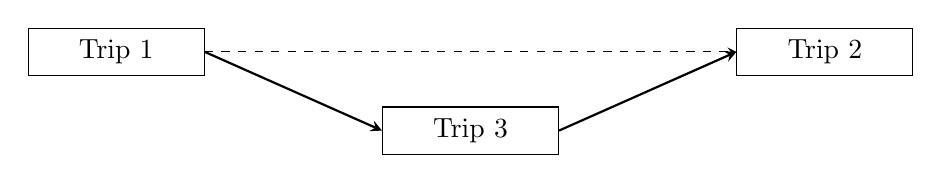
\begin{tikzpicture}[node distance=2cm]
    \node (t1) [lsnode] {Trip 1};
    \node (t2) [lsnode, xshift=9cm] {Trip 2};
    
    \node (t3) [lsnode, yshift=-1cm, xshift=4.5cm] {Trip 3};

    % Original arcs
    \draw [dashedarrow] (t1) -- (t2);

    % New arcs
    \draw [arrow] (t1.east) -- (t3.west);
    \draw [arrow] (t3.east) -- (t2.west);
  \end{tikzpicture}
  \caption{Add trip operation on the vehicle task. A new trip (in this example, trip 3) is added to the task.}
  \label{fig:addtrip-vt}
\end{figure}

\subparagraph{Remove trip} From the set of currently visited trips, select a trip $t$ at random. $t$ is then removed from $vt$, connecting its predecessor and successor via a random arc in $A_{vt}$ between the two nodes. If the resulting task is infeasible, the change is rejected. A visual representation of this operation is shown in Figure \ref{fig:removetrip-vt}.

\begin{figure}[h]
  \centering
  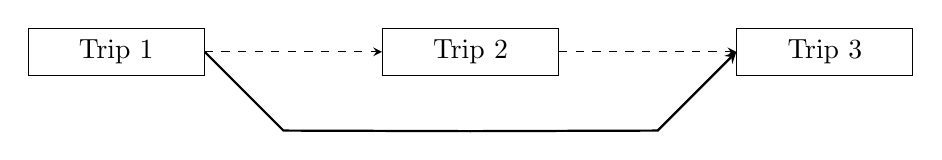
\begin{tikzpicture}[node distance=2cm]
    \node (t1) [lsnode] {Trip 1};
    \node (t2) [lsnode, xshift=4.5cm] {Trip 2};
    \node (t3) [lsnode, xshift=9cm] {Trip 3};
    
    % Original arcs
    \draw [dashedarrow] (t1) -- (t2);
    \draw [dashedarrow] (t2) -- (t3);

    % New arcs
    \draw [arrow] (t1.east) -- ($(t1.east) + (1cm, -1cm)$) -- ($(t2.south) + (0, -0.7cm)$) -- ($(t3.west) + (-1cm, -1cm)$) -- (t3.west);
  \end{tikzpicture}
  \caption{Remove trip operation on the vehicle task. An existing trip (in this example, trip 2) is removed from the task.}
  \label{fig:removetrip-vt}
\end{figure}
 
\subparagraph{Change arc} The same as the one used in the initial local search. In the vehicle task $vt$, an arc $a$ is selected at random for which at least one alternative arc exist in $A_{vt}$. $a$ is then replaced by a randomly chosen arc from the set of alternative arcs. A visual representation of this operation is shown in Figure \ref{fig:changearc-vt}. 

\noindent Any remaining SoC infeasibilities are again fixed by attempting another round of iterations with only the \textit{Change arc} operator; if this does not resolve the infeasibilities, the column is discarded. 

As with the labeling algorithm, it is interesting to include a secondary set of vehicle tasks with a different covered trip set as this may help with the final solve. In order to do this, let us take $N_{\textit{VT,LS}}$ samples of $vt$ during the simulated annealing process, distributed evenly throughout the total number of iterations performed. This results in tasks that are similar to the final result to be included in our generated set, allowing more options for inclusion in the ILP solution. These tasks are automatically discarded if they contain SoC infeasibilities, as to not waste time in an attempt to correct them.

As this local search only approximates the solution to the pricing problem, there is a chance that no task with negative reduced costs is found even if one exists. In order not to terminate the search for new columns prematurely when this happens, we instead continue for a number of column generation rounds; if a new column with negative reduced cost is found within these rounds, we continue our search. If the threshold number of rounds is reached without finding a column with negative reduced cost, we terminate the search assuming that we will not be able to improve the solution of the LP.

We also note that two different runs of this algorithm may generate different vehicle tasks, even when starting with the same dual costs. It can therefore be beneficial to run the local search multiple times in parallel during a single column generation round, allowing for a diverse set of columns to be added to the LP. 

\subsubsection{Postprocessing} \label{sec:evsp-postprocessing}
Once an integer solution is found to the E-VSP, there may still be overlap between the selected vehicle tasks. Depending on both the columns generated and the time limit given to the final solver, this number of duplicate trips may result in significant duplication of work. In order to reduce the costs incurred in driving the selected tasks, simple postprocessing is applied in order to completely eliminate any duplicate trips. 

Let us first make the assumption that for any pair of locations $l$ and $l'$ in $\mathcal{L}$, a corresponding deadhead $\mathcal{DH}$ exists. If this is not the case, temporarily extend $\mathcal{DH}$: a minimum duration and distance driven between $l$ and $l'$ using a sequence of existing deadheads and/or trips can be used as a stand-in. 

For each trip that is covered more than once, we can now select all tasks except the first which covers this trip. For each of these tasks, remove the duplicate trip from the task and replace it with a combination of a deadhead between the starting and ending location of the trip and idle time. If this results in multiple deadheads occurring without a previously planned charging operation or trip between them, combine the deadheads into one by going directly from the starting location of the first deadhead to the ending location of the last deadhead, padding with idle time when needed. This will ensure that no more SoC is used and distance is driven than in the original task, and in most cases less crew time is now required in order to complete the task.  

\subsubsection{Crew considerations}
Creation of vehicle tasks as described, while minimizing vehicle related costs, may not always result in a task which can be executed in real life. Crew members, as discussed in more detail in both Section \ref{sec:problem_def} and \ref{sec:csp-methodology}, are subject to a different set of constraints than the vehicles themselves. Most notably, crew members under most common labor regulations have a limit on continuous driving time. If a vehicle task contains a set of continuous trips without break or handover time which is longer than this limit, this immediately implies that it contains a block which no crew member is ever allowed to drive; the vehicle task itself can therefore be considered infeasible.  

Another problem arises when considering crew signing on and off for the day. In most real life instances, the number of crew bases in an area is limited. Depending on the instance, a vehicle purely minimizing driving costs may not visit these places often enough for crew members to get on and off throughout the day, also resulting in blocks that can never be driven.   

These two problems can be resolved in one of two ways: reevaluating vehicle tasks before entering the crew scheduling phase, or including some crew constraints into the feasibility of a vehicle task. The first option is known to have been used in commercial public transport planning software such as Hastus (as discussed by \citet{Hastus90}), where blocks are generated separately from the vehicle route throughout the day. We however selected the latter of the two options by adding constraints on the amount of continuous driving time and time away from a crew base to the vehicle task feasibility.

In the labeling algorithm, these values simply included in the label; they are not considered for domination rules, however they are included in the feasibility check. In both local searches, the maximum times are considered a soft constraint: going over either maximum time will incur a penalty both for the number of occurrences and the severity, once again scaling over time. If a vehicle task contains a maximum time infeasibility when iterations are done, the column is simply discarded.

\subsection{CSP} \label{sec:csp-methodology}
For the CSP, a similar approach is taken to that of the E-VSP: column generation in order to solve a set covering ILP. The set to be covered consists of the blocks present in the selected vehicle tasks. As in Section \ref{sec:evsp-methodology}, this process is broken up into steps: 
\begin{itemize}
  \item \textit{Preprocessing}, in which vehicle tasks are transformed into a set of blocks, and these blocks are in turn used to generate a graph. 
  \item \textit{Solving}, in which truncated column generation using two sources is applied in order to solve the problem of finding a set of crew duties which cover all blocks. 
\end{itemize} 
As the constraints on crew duties are significantly more complex than those of a vehicle task, we now give a short summary of the most relevant ones. For a more detailed overview and definitions of terminology we refer back to Section \ref{sec:problem_def}.

All duties consist of blocks, idle time and break time; the maximum continuous time without a break is 4 hours. Depending on the overall duration of a duty, differing amounts of break times are required. Each duty is of a certain type; this type determines acceptable start times, end times, and overall duration. A duty of type \textit{broken} includes a single long idle time, in which a crew member signs off at a crew base and then signs on again. Lastly, for an overall set of duties used to cover all blocks, constraints are in place for the percentage of long duties ($>8.5$ hours), \textit{broken} duties, \textit{between} duties and average duty length.
\subsubsection{Preprocessing}
In order to assign crew members to vehicles, the previously generated vehicle tasks must first be broken up into blocks. As defined previously in Section \ref{sec:problem_def}, a block is part of a vehicle task which must be driven by a single driver; there is no possibility of handover between drivers during the block. Let $VT$ be the collection of vehicle tasks that were previously selected. For each vehicle task $vt \in VT$, let $B_{vt}$ be the set of blocks that are contained in $vt$. The total collection of to be covered blocks $B$ can then be defined as the union of all $B_{vt}$. As with trips in the E-VSP, let each block $b \in B$ have a start time $s(b)$, end time $e(b)$, origin location $o(b)$ and destination location $d(b)$. For all blocks, both $o(b)$ and $d(b)$ are by definition relief points; a subset of all blocks may also start or end at a crew base.

Next, let us define a graph $G_{cd} = (V_{cd}, A_{cd})$ in which paths will represent crew duties. Let $V_{cd} = \{ cb_s, cb_e \} \cup B$, where $cb_s$ and $cb_e$ represent an arbitrary crew base at the start and end of a duty respectively. For every block $b \in B$ for which $o(b)$ is a crew base, add a \textit{sign-on arc} from $cb_s$ to $b$. If $d(b)$ is a crew base, add a \textit{sign-off arc} between $b$ and $cb_e$. Next, between each pair of blocks $b$ and $b'$, attempt to add an arc if $d(b) = o(b')$ and $e(b) \leq s(b')$. The type of the arc depends on $d(b)$:
\begin{itemize}
  \item If $d(b)$ is a relief point and the amount of idle time is a feasible to be a break, add a \textit{break arc}.
  \item Otherwise, if $d(b)$ is a crew base and $s(b') - e(b) - \text{sign-off/on time} \geq 1.5\text{ hours}$ add a \textit{long idle arc}. Here, the crew member signs off at the beginning of the idle time, before signing on to drive the next block. We note that given the labor regulations discussed in Section \ref{sec:problem_def}, this arc is only allowed to be used in a duty of type \textit{broken}.
  \item Otherwise, add a \textit{short idle arc}, in which the crew member remains assigned to their vehicle. 
\end{itemize}
This definition of our arcs implies that at most one arc is present between any two blocks. The number of arcs within our graph may however still be quite large; in order to reduce this, we may apply some domain knowledge in order to filter out arcs which are not part of a good solution. We will do this by enforcing minimum and maximum durations of each arc:
\begin{itemize}
  \item Sign-on/off: Any
  \item Break arcs: [0.25h, 1h]
  \item Long idle arcs: [1.5h, 5h]
  \item Short idle arcs: [0h, 0.5h]
\end{itemize} 
In this, the minimum duration of the break and long idle arcs stem from the labor regulations. We note that there are gaps within the provided thresholds; for example, an arc of 75 minutes can never be included. While this does significantly limit our number of feasible crew duties, the given bounds are realistic; creating a schedule where a crew member has a continuous paid idle time of longer than an hour will rarely occur in practice.

Any feasible crew duty can now be represented as a path between $cb_s$ and $cb_e$ in $G_{cd}$. We again note that not every path from $cb_s$ to $cb_e$ represents a feasible duty; based on the chosen duty type, differing combinations of duty length, break times and idle times might be feasible.   
\subsubsection{Solving}
Similarly to our model for the E-VSP, let us define a set covering ILP in order to find a set of feasible crew duties which cover all to be driven blocks. In this, let $\textit{CD}$ be the available crew duties, let $y_j$ be a binary decision variable indicating the usage of $cd_j \in \textit{CD}$, and let $m_{j,b}$ be a parameter indicating that crew duty $cd_j$ covers block $b \in B$. In order to model the constraints on the overall set of duties, let us introduce an additional set of parameters. Let $d_j$ be the total working duration of duty $cd_j$, let $d_{j,\textit{long}}$ indicate that $d_j$ is longer than 8.5 hours, and let $\rho_{j,\textit{broken}}$ and $\rho_{j,\textit{between}}$ indicate that $cd_j$ is of duty type \textit{broken} or \textit{between}, respectively. We can then define our ILP as follows:
\begin{align}
\min \quad
& \sum_{cd_j \in \textit{CD}} y_{j} \cdot cost(cd_j)
\end{align}
Subject to:
\begin{align}
\sum_{cd_j \in \textit{CD}} y_{j}m_{j,b} &\geq 1 && \forall b \in B \label{form:block-cover}\\
\sum_{cd_j \in \textit{CD}} y_{j} \cdot (\frac{d_{j}}{\textit{8 hours}} - 1) &\leq 0 && \label{form:max-avg-shift-length}\\
\sum_{cd_j \in \textit{CD}} y_{j} \cdot (0.15 - d_{j,\textit{long}}) &\geq 0 && \label{form:max-long-shifts}\\
\sum_{cd_j \in \textit{CD}} y_{j} \cdot (0.3 - \rho_{j,\textit{broken}}) &\geq 0 && \label{form:max-broken-shifts}\\
\sum_{cd_j \in \textit{CD}} y_{j} \cdot (0.1 - \rho_{j,\textit{between}}) &\geq 0 && \label{form:max-between-shifts}\\
y_{j} &\in \{ 0, 1 \} && \forall cd_j \in \textit{CD} \label{form:y-integer}
\end{align}
Here, constraint (\ref{form:block-cover}) ensures that all blocks are covered, constraint (\ref{form:max-avg-shift-length}) ensures a maximum average duty length, constraint (\ref{form:max-long-shifts}) ensures that a max of 15\% of all selected shifts is long, and constraints (\ref{form:max-broken-shifts}) and (\ref{form:max-between-shifts}) ensure that a maximum of 30\% of selected duties are of type \textit{broken} and 10\% are of type \textit{between} respectively. In this, we note that constraint (\ref{form:block-cover}) allows for overcoverage of blocks, increasing the overall solution space. If a solution is found where multiple drivers are assigned to the same block, all but one of the drivers can simply be passengers for the duration of the block. 

This problem can be relaxed to an LP by replacing constraint (\ref{form:y-integer}) with the following:
\begin{align}
0 &\leq y_{j} && \forall cd_j \in \textit{CD}
\end{align}
In this relaxed problem, let the dual cost of constraints (\ref{form:block-cover}-\ref{form:max-between-shifts}) be $\tau_{b}, \tau_{\textit{avg}}, \tau_{\textit{long}}, \tau_{\textit{broken}}$ and $\tau_{\textit{between}}$ respectively. Using this, we can define the reduced costs of a new crew duty $cd_0$ as being: 
\begin{align}
\text{cost}(cd_0) 
&- \sum_{b \in B} m_{0,b} \tau_{b} 
- \frac{d_0}{\text{8 hours}} \tau_{\textit{avg}} \nonumber \\
&- \tau_{\textit{long}} (0.15 - d_{0,\textit{long}}) 
- \tau_{\textit{broken}} (0.3 - \rho_{0,\textit{broken}}) 
- \tau_{\textit{between}} (0.1 - \rho_{0,\textit{between}})
\end{align}

An initial set of columns for the LP relaxation can once again be found by running a number of local searches, each of which attempts to cover all blocks. After this initial set, the pricing problem is again repeatedly solved using a labeling algorithm; this is repeated until the relaxed problem is solved to optimality or until a predefined time limit is hit. Finally, constraint (\ref{form:y-integer}) is reinstated, and an integer solution is found using branch-and-bound.

\paragraph{Initial solution - Local search}
As with the E-VSP, an initial set of crew duties can be constructed using a simulated annealing algorithm. In this, let us start with a set of crew duties each containing exactly one block. As crew duties must have a duty type, a type which is feasible given the start and end time of the block is randomly selected. We note that this initial solution may not be feasible as a whole, as the start and end locations of blocks are not required to be a crew base. In order to deal with this, we apply a penalty to each duty which does not start and end at a crew base. Additionally, constraints (\ref{form:max-avg-shift-length}-\ref{form:max-between-shifts}) are each relaxed by applying a penalty if the overall set of duties does not satisfy the constraint. This penalty is based on a percentage difference between the target and value in the duty set.

Next, the following set of operations is applied in order to recombine the duties. We note that the operators used in this local search are almost identical to those described earlier in Section \ref{sec:evsp-initial-local-search}. The key difference is the use of blocks as the main elements within a duty as opposed to trips for a vehicle task. We will therefore refer back to the illustration provided earlier for a visual representation of the operations, substituting trips for blocks and tasks for duties where applicable. Similarly to the E-VSP local searches, it can also be beneficial to include the unfiltered arcs during the search in order to allow for longer breaks/idle time, thereby increasing the solution space.

\noindent\subparagraph{2-Opt (or tail swap)} Two different duties $cd$ and $cd'$ are selected at random from the available set of duties. Next, a time $t$ between the minimum start and maximum end time of $cd$ and $cd'$ is selected. All blocks after $t$ in $cd$ are moved to $cd'$, while at the same time moving all blocks after $t$ in $cd'$ to $cd$. If no arcs in $A_{cd}$ exist to reconnect the swapped tails of the duties, the change is rejected. If the resulting schedules contain a different infeasibility (such as a start or end time which conflicts with the current duty type), an additional check is done to see if changing a duty type might make the change feasible. A new duty is then selected from the list of feasible duty types, prioritizing types which are not constrained. If this is not possible, the change is rejected. If one of the duties becomes empty due to the operation, it is removed from the set of available duties. A visual representation can be found in Figure \ref{fig:2opt-vt}.
\noindent\subparagraph{Range move} Two different duties $cd$ and $cd'$ are selected at random from the available set of duties. Next, from $cd'$, a random continuous range of blocks $r$ is selected; $r$ is removed from $cd'$ and is added to $cd$. If no arcs exist to connect $r$ in $cd$ or remove $r$ from $cd'$, the change is rejected. Next, as with 2-Opt, an attempt is made to make the duties feasible by changing the types; if this fails, the change is rejected. If $cd'$ becomes empty due to the operation, it is removed from the set of available duties. A visual representation can be found in Figure \ref{fig:rangemove-vt}.
\noindent\subparagraph{Single block move} Same as the range move, however we now only select a single block from $cd'$. This is done as blocks can be quite long, therefore moving a range might be difficult if it contains a single long block. \\

\noindent After termination, the generated duties may still be infeasible if the soft constraints are still violated. This can either be because the set of generated duties does not match the duty type / duration requirements, or because some of the duties do not properly start or end at a crew base. In order to resolve both of these problems, a set of dummy columns is added to the LP formulation: each covers exactly one block without any constraints, however the use of one of these columns is discouraged by giving it significant costs. This still allows for a solution to the LP relaxation to be found, allowing for dual costs to be determined. This in turn allows the column generation phase to resolve the remaining uncovered blocks.

\paragraph{Pricing problem - Labeling}
Let us consider our previously defined graph $G_{cd} = (V_{cd}, A_{cd})$. As with the labeling algorithm described in the E-VSP section, we can once again attempt to find a path of minimum cost through our graph $G_{cd}$ in order to generate a crew duty with minimum reduced cost. In order to do this, we once again modify the costs of the arcs in $A_{cd}$ in order to include the dual costs, adding the dual cost for duty length and type during the evaluation of $cb_e$. For a more detailed overview of the algorithm, we refer to Section \ref{sec:labeling-evsp}, however we will discuss details specific to label propagation in the crew duty variant here. 

We now start with a set of empty labels in $cb_s$, one for each available duty type. During propagation, in each label keep track of:
\begin{itemize}
  \item The duty type of the label.
  \item The previous label.
  \item The starting time of the duty, defined by the first duty after $cb_s$.
  \item The breaks arcs taken in this duty.
  \item The long idle arcs taken in this duty.
\end{itemize}
Clear domination rules are not present, as the accrued reduced costs are only dominated if start time, breaks, idles and duty type are identical. As this is unlikely, removing as many labels as possible through feasibility constraints remains as the best option to ensure that computational efficiency is maintained.

Checking for feasibility during propagation can however only be done for a subset of the provided labor regulations. Properties such as overall duty duration, continuous driving time, minimum start and maximum end time, and use of long idle arcs can already be used in order to remove labels which cannot result in a feasible duty of a given type. Before reaching $cb_e$ however, the end time and distribution of breaks in the duty are not yet finalized. This notably implies that it is not possible to check for sufficient breaks while propagation is still in progress. As an example, suppose some label in the process indicates that its corresponding duty will have a length of at least 6 hours, requiring a total of 40 minutes of break time under Dutch labor regulations. If the current amount of break time is 20 minutes, this may still become feasible before reaching $cb_e$ by taking another break arc; we can therefore not discard this label before knowing that the duty has ended.  

Once propagation has completed, the duties described by the labels in $cb_e$ can be finalized. Only then can we do our full feasibility check, discarding any labels which are not valid given their state in $cb_e$. As with the E-VSP, what remains is a list of labels which describe feasible duties which can be sorted on non-decreasing reduced cost. We will then take at most $N_{\textit{CD,LB}}$ of these duties with negative reduced cost, prioritizing block-disjoint duties. Next, secondary columns are generated for the best $M_{\textit{CD,LB}} \leq N_{\textit{CD,LB}}$ of the found duties. After this, the complete set of duties is made available to the LP relaxation, before repeating the process with new values of $\tau$. 

\subsection{E-VCSP}
In order to solve the E-VCSP, we will reuse large parts of the techniques used in Section \ref{sec:evsp-methodology} and \ref{sec:csp-methodology}. We will once again break this problem up into steps: 
\begin{itemize}
  \item \textit{Initial solution}, in which a baseline solution is found by solving the E-VSP and CSP sequentially.
  \item \textit{Solution improvement}, in which column generation is applied in an attempt to find a better solution given the interaction between the vehicle and crew.
\end{itemize}

\subsubsection{Initial solution}
In order to have a baseline solution for the E-VCSP, we first solve the E-VSP and CSP sequentially using the techniques discussed in Sections \ref{sec:evsp-methodology} and \ref{sec:csp-methodology}. 

During the solving process, a set of columns $VT$ and $CD$ representing vehicle tasks and crew duties respectively are generated. Let $VT^* \subseteq VT$ and $CD^* \subseteq CD$ be the selected subsets that form the solution to the sequential problem, with $z^*$ being the total cost of this solution; this will be used to provide an upper bound to the solution quality of the integrated problem. 

\subsubsection{Solution improvement}
We will now attempt to improve the initial solution. In order to do this, we will first discuss some modifications to how we view blocks in our solution. Using this, we will provide an ILP formulation for the E-VCSP and discuss the problems that arise by directly using its corresponding LP relaxation. Then, we will give a Lagrangean relaxation of the ILP with which the E-VCSP was solved. We will then discuss the modifications needed to the column generations methods from Sections \ref{sec:evsp-methodology} and \ref{sec:csp-methodology} in order to use them for the integrated problem. Lastly, we will discuss additional heuristics which were applied in order to maintain computational efficiency. 

\paragraph{Block redefinition} During our sequential approach, we assumed that all blocks given to the CSP were unique. This is generally the case, as after postprocessing of the E-VSP solution, no two blocks share the same trip. It could still occur that two vehicles were scheduled to drive the same deadhead at the same time, possibly resulting in two identical blocks containing only a deadhead; this was exceedingly rare during testing, and was therefore handled by still considering the two blocks as separate.

When no postprocessing is applied however, blocks containing the same content may occur much more frequently. Additionally, we will soon see that we want to consider all blocks in the available set of vehicle tasks, not just blocks in tasks which are selected in a final solution. It is therefore highly likely that duplicate blocks occur within our set of available vehicle tasks. As we do not want to consider these as separate blocks when constructing crew duties, we will now define an equality relation for our blocks. 

Let us do this by considering how blocks are used in the crew solution. Here, a block is simply a working period with a start location, start time, end location and end time. The contents themselves do not influence the feasibility of a duty, as a crew member is already assumed to be working for the duration of the block. Going forward, let us therefore consider any two blocks that share a start location, start time, end location and end time to be equal, even if the contents are different. This allows us to now create duties over blocks without knowing their exact contents, resulting in duties which can be reused when blocks occur in a different vehicle task. 

\paragraph{ILP formulation and LP relaxation} Let us now define an ILP which can be used in order to solve the E-VCSP. We will largely follow the same formulation as previously discussed in Sections \ref{sec:problem_def}, \ref{sec:evsp-methodology} and \ref{sec:csp-methodology}, however we will make slight adjustments in order to incorporate our new block definition. 

Let $VT$ and $CD$ be the sets of available vehicle tasks and crew duties respectively. Next, let $B_{vt}$ be the blocks covered by vehicle task $vt \in VT$, and let $B_{cd}$ be defined similarly. Let $B = \bigcup_{vt \in VT} B_{vt} \cup \bigcup_{cd \in CD} B_{cd}$ be the set of \emph{known blocks}, or put simply the set of blocks which are present in at least one generated column. In this, we use our new definition of block equality in order to construct the overall set of known blocks. 

Let $x_i$ and $y_j$ be binary and integer decision variables indicating the usage of vehicle task $vt_i \in VT$ and crew duty $cd_j \in CD$ respectively. Let $k_{i,t}$, $l_{i,b}$ and $m_{j,b}$ be parameters indicating that $vt_i$ covers $t$, $vt_i$ contains block $b$ and $cd_j$ covers $b$ respectively, again using the new definition of block equality. Additionally, let $d_j$ be the duration of $cd_j$, let $d_{j,\textit{long}}$ indicate that $d_j$ is longer than 8.5 hours, and let $\rho_{j,\textit{broken}}$ and $\rho_{j,\textit{between}}$ indicate that $cd_j$ is of duty type \textit{broken} or \textit{between}, respectively. Lastly, let $cost(vt_i)$ and $cost(cd_j)$ be the costs of vehicle task $vt_i$ and crew duty $cd_j$ respectively. Our ILP is then defined as follows:

\begin{align}
\min \quad
& \sum_{vt_i \in VT} x_{i} \cdot cost(vt_i) + \sum_{cd_j \in CD} y_{j} \cdot cost(cd_j)  
\end{align}
Subject to:
\begin{align}
\sum_{vt_i \in VT} x_{i}k_{i,t} &\geq 1 && \forall t = 1,\:\dots,\:|T| \label{form:methods-integrated-all-trips-covered} \\
\sum_{vt_i \in VT}x_i l_{i,b} - \sum_{cd_j \in CD}y_j m_{j,b} &\leq 0 && \forall b \in B \label{form:methods-integrated-all-blocks-covered} \\
\sum_{cd_j \in \textit{CD}} y_{j} \cdot (\frac{d_{j}}{\textit{8 hours}} - 1) &\leq 0 && \label{form:methods-integrated-max-avg-shift-length}\\
\sum_{cd_j \in \textit{CD}} y_{j} \cdot (0.15 - d_{j,\textit{long}}) &\geq 0 && \label{form:methods-integrated-max-long-shifts}\\
\sum_{cd_j \in \textit{CD}} y_{j} \cdot (0.3 - \rho_{j,\textit{broken}}) &\geq 0 && \label{form:methods-integrated-max-broken-shifts}\\
\sum_{cd_j \in \textit{CD}} y_{j} \cdot (0.1 - \rho_{j,\textit{between}}) &\geq 0 && \label{form:methods-integrated-max-between-shifts}\\
x_{i} &\in \{ 0, 1 \} && \forall vt_i \in VT \\
y_{j} &\in \mathbb{N}_0 && \forall cd_j \in CD
\end{align}
In this, constraint (\ref{form:methods-integrated-all-trips-covered}) ensures that all trips are covered by at least one vehicle task. Constraint (\ref{form:methods-integrated-all-blocks-covered}) ensures that there are enough drivers available for all blocks used in vehicle tasks. Constraints (\ref{form:methods-integrated-max-avg-shift-length}-\ref{form:methods-integrated-max-between-shifts}) once again ensure that average shift length and shift type constraints resulting from the labor regulations are met.

We note that constraints (\ref{form:methods-integrated-all-trips-covered}) and (\ref{form:methods-integrated-all-blocks-covered}) allow overcoverage; that is, a trip can be driven more than once, and a block may be covered by more drivers than vehicles. When a trip is driven multiple times, any unnecessary buses may simply drive a deadhead instead. When more drivers are assigned to a block than vehicles, all additional drivers may simply ride along as passengers. 

Under this formulation, it is also possible that a driver is assigned to a block which is not driven; in this case, an alternate form of transport would need to be used in order to get the driver from the starting location to the ending location of the block. In our testing, this almost never occurred in final solutions due to the associated increase in crew cost, and in the following sections we will therefore assume that a final schedule does not contain this type of conflict. Note that one might also choose to introduce a cost penalty when this occurs, modeling the costs of the alternate form of transport.

This ILP may once again be relaxed to an LP by removing the binary / integrality constraints of $x$ and $y$. Solving this LP gives us a set of dual costs for the constraints (\ref{form:methods-integrated-all-trips-covered}-\ref{form:methods-integrated-max-between-shifts}), which we shall refer to as $\pi_t,\:\pi_b,\:\pi_{avg},\:\pi_{long},\:\pi_{between}$ and $\pi_{broken}$ respectively. Using this, we now define the reduced cost for a vehicle task $vt_0$ as being:
\begin{align}
\text{cost}(vt_0) - \sum_{t \in T} k_{0,t}\pi_t - \sum_{b \in B} l_{0,b}\pi_b \label{form:evcsp-rc-vt}
\end{align}
As we can see, the dual cost $\pi_b$ of the blocks contained in $vt_0$ now influence the reduced cost of the task; the quality of the crew solution is therefore now linked to the reduced cost of a vehicle task.

For a crew duty $cd_0$, we can similarly define the reduced cost as follows: 
\begin{align}
\text{cost}(cd_0) 
&+ \sum_{b \in B} m_{0,b} \tau_{b} 
- \frac{d_0}{\text{8 hours}} \tau_{\textit{avg}} \nonumber \\
&- \tau_{\textit{longdur}} (0.15 - d_{0,\textit{long}}) 
- \tau_{\textit{broken}} (0.3 - \rho_{0,\textit{broken}}) 
- \tau_{\textit{between}} (0.1 - \rho_{0,\textit{between}})
\end{align}
Note that this formulation is almost identical to the one found in Section \ref{sec:csp-methodology}, however the sign for the contribution of the block dual costs is flipped due to the change in sign in the LP formulation. 

Using these reduced cost formulations, we can now once again apply column generation to find columns with negative reduced cost which will improve the solution quality of our LP. In order to do this, we will alternate between finding vehicle and crew columns. After doing this for a number of rounds, integrality constraints are reinstated and branch-and-bound is used to find a final solution. An outline of the approach is given in Algorithm \ref{alg:E-VCSP-rounds-lp}. 

\begin{algorithm}[h]
\caption{E-VCSP Rounds - LP}\label{alg:E-VCSP-rounds-lp}
\begin{algorithmic}[1]
\State $(VT, CD) \gets \Call{SequentialSolution}$
\State $(x, y, \pi) \gets \Call{SolveLP}{VT, CD}$
\For{$round \in 1 ... MaxRounds$} 
  \For{$i \in 1 \dots N_{VT}$}
    \State $VT \gets VT \cup \Call{GenVTs}{T, \pi}$
    \State $(x, y, \pi) \gets \Call{SolveLP}{VT, CD}$
  \EndFor
  \For{$i \in 1 \dots N_{CD}$}
    \State $B' \gets$ Blocks covered by vehicle tasks in $VT$ with $x_i > 0$ \label{line:block-coverage}
    \State $CD \gets CD \cup \Call{GenCDs}{B', \pi}$
    \State $(x, y, \pi) \gets \Call{SolveLP}{VT, CD}$
  \EndFor
\EndFor
\State{$(x,y,z) \gets \Call{SolveILP}{VT,CD}$}
\end{algorithmic}
\end{algorithm}

Initial testing using this round based approach showed poor results; the columns generated during the round did not lead to significant improvements to the final (integer) solution. 

On the crew side, this can most likely be traced back to Algorithm \ref{alg:E-VCSP-rounds-lp} line {\ref{line:block-coverage}}; here, a selection is made from all known blocks in order to use as a basis for duty generation based on the blocks currently present in (partially) selected tasks. This both gives an indication that a block is more likely to be useful in the final solution and limits the overall number of blocks in $B'$. In our initial experiments however, it became apparent that the number of blocks in $B'$ was generally still rather large, often exceeding twice the number of blocks considered during the sequential problem. This resulted in generated duties with blocks that were unlikely to occur in final solutions, thereby reducing the effectiveness of the generation as a whole.

The same argument partially applies to the generation of vehicle tasks: blocks in duties which were unlikely to occur in final solutions could be partially selected, resulting in dual costs for these blocks which can negatively influence the direction of vehicle task column generation. 

\paragraph{Lagrangean relaxation}
In order to resolve the issues that arise from directly using the LP relaxation, let us instead apply a Lagrangean relaxation to our original ILP. In this, we replace constraints with penalties in the objective function when the constraint is not met. This allows us to fully relax the block linking constraint (\ref{form:methods-integrated-all-blocks-covered}), allowing us to once again consider the vehicle and crew parts as separate problems. 

Previous work by \citet{vanKootenNiekerk2017} has also shown that relaxing the trip coverage constraint (\ref{form:methods-integrated-all-trips-covered}) leads to a problem which is computationally easier to solve while maintaining high quality final solutions. As such, we have decided to fully relax our problem. That is, constraints (\ref{form:methods-integrated-all-trips-covered}-\ref{form:methods-integrated-max-between-shifts}) are all relaxed. For each relaxed constraint, let us define our penalty factor (more commonly known as a Lagrangean multiplier $\lambda$) and contribution to the objective function as follows: 
\begin{align}
\lambda_{t} &\geq 0 && \lambda_{t} (1 - \sum_{vt_i \in VT} x_{i}k_{i,t}) && \forall t = 1,\:\dots,\:|T| \nonumber \\
\lambda_{b} &\geq 0 && \lambda_{b} (\sum_{vt_i \in VT} x_i l_{i,b} - \sum_{cd_j \in CD}y_j m_{j,b}) && \forall b \in B \nonumber \\
\lambda_{\text{avg}} &\geq 0 && \lambda_{\text{avg}} (\sum_{cd_j \in \textit{CD}} y_{j} \cdot (\frac{d_{j}}{\textit{8 hours}} - 1)) && \nonumber \\
\lambda_{\text{long}} &\geq 0 && -\lambda_{\text{long}} (\sum_{cd_j \in \textit{CD}} y_{j} \cdot (0.15 - d_{j,\textit{long}})) && \nonumber \\
\lambda_{\text{broken}} &\geq 0 && -\lambda_{\text{broken}} (\sum_{cd_j \in \textit{CD}} y_{j} \cdot (0.3 - \rho_{j,\textit{broken}})) && \nonumber \\
\lambda_{\text{between}} &\geq 0 && -\lambda_{\text{between}} (\sum_{cd_j \in \textit{CD}} y_{j} \cdot (0.1 - \rho_{j,\textit{between}})) && \nonumber
\end{align}
Let us refer to the collection of these multipliers as simply $\lambda$. Given a multiplier set $\lambda$, we can now redefine our objective function as follows:
\begin{align}
\min \quad
& \sum_{vt_i \in VT} x_{i} \cdot cost(vt_i) + \sum_{cd_j \in CD} y_{j} \cdot cost(cd_j)\quad+ \nonumber \\ 
&\lambda_{t} (1 - \sum_{vt_i \in VT} x_{i}k_{i,t}) + \lambda_{b} (\sum_{cd_j \in CD}y_j m_{j,b} - \sum_{vt_i \in VT}x_i l_{i,b}) \quad+\nonumber \\
&\lambda_{\text{avg}} (\sum_{cd_j \in \textit{CD}} y_{j} \cdot (\frac{d_{j}}{\textit{8 hours}} - 1)) -\lambda_{\text{long}} (\sum_{cd_j \in \textit{CD}} y_{j} \cdot (0.15 - d_{j,\textit{long}}))\quad- \nonumber \\
&\lambda_{\text{broken}}(\sum_{cd_j \in \textit{CD}} y_{j} \cdot (0.3 - \rho_{j,\textit{broken}})) -\lambda_{\text{between}} (\sum_{cd_j \in \textit{CD}} y_{j} \cdot (0.1 - \rho_{j,\textit{between}})) \nonumber
\end{align}
Which we can simplify to the following:
\begin{align}
\min \quad & \sum_{vt_i \in VT} x_{i} (cost(vt_i) -\sum_{t \in T} \lambda_{t} k_{i,t} - \sum_{b \in B} \lambda_{b} l_{i,b})\quad+ \nonumber \\
& \sum_{cd_j \in CD} y_{j} (cost(cd_j) + \sum_{b \in B} \lambda_{b} m_{j,b} + \lambda_{\text{avg}} (\frac{d_{j}}{\textit{8 hours}} - 1) - \lambda_{\text{long}} (0.15 - d_{j,\text{long}}) \nonumber \\
&\quad\quad\quad\quad\:-\lambda_{\text{broken}} (0.3 - d_{j,\text{broken}}) - \lambda_{\text{between}} (0.1 - d_{j,\text{between}})) \quad + \nonumber \\
& \sum_{t \in T} \lambda_{t} \nonumber
\end{align}
In this, we note that for a given set of multipliers $\lambda$, the costs for selecting a vehicle task or crew duty are fixed; let us define the cost of a vehicle task $vt_i$ and crew duty $cd_j$ under multipliers $\lambda$ as being $cost_\lambda(vt_i)$ and $cost_\lambda(cd_j)$ respectively. Our problem, given a fixed $\lambda$, can now be written as follows:
\begin{align}
\min \quad \sum_{vt_i \in VT}& x_{i} \cdot cost_\lambda(vt_i) + \sum_{cd_j \in CD} y_{j} \cdot cost_\lambda(cd_j) + \sum_{t \in T} \lambda_{t}
\end{align}
\begin{align}
x_{i} &\in \{ 0, 1 \} && \forall vt_i \in VT \\
 y_{j} &\in \mathbb{N}_0 && \forall cd_j \in CD
\end{align}
For a given set of multipliers $\lambda$, we can now find a solution to the problem by inspection. First, for all $vt_i \in VT$ for which $cost_\lambda(vt_i) < 0$, set $x_i = 1$ otherwise $x_i = 0$. This is guaranteed to be optimal as the inclusion of any other vehicle task will by definition only increase the overall cost of the solution. 

For the duties, we cannot directly do the same as $y_j$ has no upper bound. We can however apply a heuristic in order to set an upper bound of $y_j$, after which we can apply a similar technique. In order to do this, let $\textit{count}_x(b)$ represent the number of times block $b \in B$ is covered given the currently selected set of vehicle tasks $x$. Next, let $B_{cd_j}$ represent the blocks covered by $cd_j$; we can then define our upper bound $\bar{y_{j}}$ of $y_j$ as being $\max \{ \textit{count}_x(b)\:|\:b \in B_{cd_j} \} \cup \{ 1 \}$; that is, the maximum number of times the duty may be selected without causing guaranteed overcoverage of blocks, with a minimum of 1. 

Using this, for all $cd_j \in CD$ for which $cost_\lambda(cd_j) < 0$, set $y_j = \bar{y_{j}}$, otherwise $y_j = 0$, following the same reasoning as earlier. We can ignore the $\lambda_t$ term as it is constant for a given set of multipliers.

The solution of this Lagrangean relaxation provides a lower bound to the optimal solution of the original E-VCSP. The quality of this lower bound may differ depending on the value of $\lambda$. In order to find the best lower bound, we would need to solve the following problem:
\begin{align}
\max_{\lambda} \quad & \min \sum_{vt_i \in VT} x_{i} \cdot cost_\lambda(vt_i) + \sum_{cd_j \in CD} y_{j} \cdot cost_\lambda(cd_j) + \sum_{t \in T} \lambda_{t}
\end{align}
Let $\lambda^*$ be the set of multipliers for which our lower bound is maximized. $\lambda^*$ can be used as a stand-in for the dual values $\pi$ of the LP relaxation discussed in the previous section, allowing us to once again use the column generation methods that we used in the sequential problem. In order to find $\lambda^*$, we use subgradient optimization; during this process, we start with an initial set of multipliers, updating them in rounds in order to find a better lower bound to the relaxed problem. We refer to \citet{Beasley1993} for exact implementation details. \todo{Is het handig om hier nog in te gaan op details?}

We note that during our relaxation, we said that $\lambda_b \geq 0$; this would imply that using a block could only have a positive influence on a vehicle task which includes it, as the multiplier is subtracted from the reduced costs. It may also be beneficial for a crew solution to be able to discourage the use of a block, therefore let us instead say that $\lambda_b \in \mathbb{R}$ for all $b$. This is equivalent to making constraint (\ref{form:methods-integrated-all-blocks-covered}) an equality in our relaxation. 

As a consequence, the relaxation no longer provides a direct lower bound to the solution quality; an exact block cover may be more expensive than an overcoverage with the available sets of vehicle and crew schedules. We do however know that in a final solution, overcoverage is undesirable as this results in higher variable crew costs. Finding a $\lambda^*$ which steers towards no overcoverage is therefore still useful.

Using $\lambda^*$ as a stand-in for our dual costs does have another drawback: columns which are already known may be generated, as columns in the basis may get negative reduced cost. In order to minimize this effect, we will apply a modified version of a heuristic previously used by \citet{vanKootenNiekerk2017, Freling1997, Carraresi1995} which adjust the multipliers such that all selected columns have a nonnegative reduced cost, and the value of the relaxation does not decrease. We separately apply this heuristic for vehicle columns or crew columns, depending on which type of columns we will be generating in a given round.
\begin{algorithm}[h]
\caption{Lagrangean Multiplier Heuristics}\label{alg:lagrange-multiplier-vt}
\begin{algorithmic}
\Procedure{NonNegativeVTs}{$VT, \lambda$} \Comment{Adjust Vehicle Task Multipliers}
\For{$vt_i \in VT,\:cost_\lambda(vt_i) < 0$} 
  \State $\delta \gets cost_\lambda(vt_i) / (\sum_{t \in T} k_{i,t} + \sum_{b \in B} l_{i,b})$
  \For {$t \in T,\:k_{i,t} = 1$}
    \State $\lambda_{t} \gets \lambda_{t} + \delta$
  \EndFor
  \For {$b \in B,\:l_{i,b} = 1$}
    \State $\lambda_{b} \gets \lambda_{b} + \delta$
  \EndFor
\EndFor

\Return $\lambda$
\EndProcedure\\
\Procedure{NonNegativeCDs}{$CD, \lambda$} \Comment{Adjusts Crew Duty Multipliers}
  \For{$cd_j \in CD,\:cost_\lambda(cd_j) < 0$} 
    \State $\delta \gets cost_\lambda(cd_j) / (0.55 - \sum_{b \in B} m_{j,b} - (\frac{d_{j}}{\textit{8 hours}} - 1) - d_{j,\textit{long}} - \rho_{j,\textit{broken}} - \rho_{j,\textit{between}})$
    \For {$b \in B,\:m_{j,b} = 1$}
      \State $\lambda_{b} \gets \lambda_{b} + \delta$
    \EndFor
    \State $\lambda_{avg} \gets \lambda_{avg} + \delta$
    \State $\lambda_{long} \gets \lambda_{long} + \delta$
    \State $\lambda_{broken} \gets \lambda_{broken} + \delta$
    \State $\lambda_{between} \gets \lambda_{between} + \delta$
  \EndFor

\Return $\lambda$
\EndProcedure
\end{algorithmic} 
\end{algorithm}

We now have a method to find approximated dual costs for each of the constraints by letting $\pi \gets \lambda$. We will now modify Algorithm \ref{alg:E-VCSP-rounds-lp} in order to use this new approach. An outline of this process has been provided in Algorithm \ref{alg:E-VCSP-lagrange}.

\begin{algorithm}
\caption{E-VCSP Rounds - Lagrangean}\label{alg:E-VCSP-lagrange}
\begin{algorithmic}
\State $(VT, CD, z_{init}) \gets \Call{SequentialSolution}$
\State $(x, y, \lambda) \gets \Call{SubgradientOpt}{VT, CD}$
\While{$round \in 1 ... MaxRounds$} 
  \For{$i \in 1 \dots N_{VT}$}
    \State $\lambda \gets$ \Call{NonNegativeVTs}{$VT, \lambda$}
    \State $VT \gets VT \cup \Call{GenVTs}{T, \lambda}$
    \State $(x, y, \lambda) \gets \Call{SubgradientOpt}{VT, CD}$
  \EndFor
  \For{$i \in 1 \dots N_{CD}$}
    \State $B' \gets$ Blocks covered by vehicle tasks in $VT$ with $x_i = 1$
    \State $\lambda \gets$ \Call{NonNegativeCDs}{$CD, \lambda$}
    \State $CD \gets CD \cup \Call{GenCDs}{B', \lambda}$
    \State $(x, y, \lambda) \gets \Call{SubgradientOpt}{VT, CD}$
  \EndFor
\EndWhile
\end{algorithmic}
\end{algorithm}

\paragraph{Column generation} \label{sec:evcsp-cg}
In order to improve our solution quality beyond the initial sequential solution, we once again apply column generation. However, as we have split the integrated problem into two separate subproblems by relaxing the block link constraint, we can reuse the column generation methods that we discussed in Sections \ref{sec:evsp-methodology} and \ref{sec:csp-methodology}. As our formulas for reduced costs have slightly changed, our generation methods will be modified slightly in order to incorporate these changes.

\subparagraph{E-VSP Labeling} Let us recall the reduced cost formula for a vehicle task $vt_0$ as described by Formula (\ref{form:evcsp-rc-vt}). As mentioned earlier, the difference between this and the reduced cost formula in the sequential problem is the inclusion of the dual costs of the blocks which are contained within the vehicle task. 

In order to incorporate these costs in our labeling algorithm, let us first visualize known blocks within our graph $G_{vt}$ by outlining them; see Figure \ref{fig:evsp-graph-blocks} for an example. As before, we represent the ends of trips as nodes and the connecting arcs incorporate both movements and (charging) idles. As blocks may start and end whenever a sufficiently long idle period is present at a relief point, the borders of blocks will always fall somewhere within an edge.  

\begin{figure}[h]
  \centering
  \begin{tikzpicture}[
    node distance=25mm and 18mm,
  ]
  % Nodes
  \node[lsnode] (A) {Trip 1};
  \node[lsnode, right=25mm of A, yshift=-10mm] (B) {Trip 2};
  \node[lsnode, right=25mm of B, yshift=10mm] (C) {Trip 3};
  \node[lsnode, right=25mm of B, yshift=-10mm] (D) {Trip 4};

  \draw[->] (B.east) -- (C.west);
  \draw[->] (B.east) -- (D.west);
  \draw[-] (A.east) -- (B.west);
  \draw[-] ($(A.west) + (0,-24mm)$) -- (B.west);
  \draw[->] ($(B.west) + (-0.01mm, 0)$)-- (B.west);
  % \draw[->] (B.east) -- ++(63mm,0);
  \draw[->] (C.east) -- ++(15mm,0);
  \draw[->] (D.east) -- ++(15mm,0);

  \draw[dash pattern={on 1pt off 2pt}, thick, rounded corners=8pt]
    ($(A.east) + (0,-17.5mm) +(0mm,6mm)$) -- ($(B.north west)+(-3mm,3mm)$) -- ($(B.north east)+(3mm,3mm)$) -- ($(C.north west)+(-3mm,3mm)$) -- ($(C.north east)+(0mm,3mm)$) -- ($(C.south east)+(0mm,-3mm)$) -- ($(C.south west)+(-3mm,-3mm)$) -- ($(B.south east)+(3mm,-3mm)$) -- ($(B.south west)+(-3mm,-3mm)$) -- ($(A.east) + (0,-17.5mm) +(0mm,-6mm)$) -- cycle;
  \draw[dashed, thick, rounded corners=8pt]
    ($(A.north east)+(0mm,3mm)$) -- ($(B.north west)+(-3mm,3mm)$) -- ($(B.north east)+(3mm,3mm)$) -- ($(D.north west)+(-3mm,3mm)$) -- ($(D.north east)+(0mm,3mm)$) -- ($(D.south east)+(0mm,-3mm)$) -- ($(D.south west)+(-3mm,-3mm)$) -- ($(B.south east)+(3mm,-3mm)$) -- ($(B.south west)+(-3mm,-3mm)$) -- ($(A.south east)+(0mm,-3mm)$) -- cycle;
  \node[above=3mm of C.north] {Block 1};
  \node[below=3mm of D.south] {Block 2};
  \end{tikzpicture}
  \caption{A simplified view of $G_{vt}$ with 2 known blocks. Trip nodes represent ends of trips, edges contain both movements and idles between pairs of trips.}
  \label{fig:evsp-graph-blocks}
\end{figure}

Suppose that in this graph, we have two labels in Trip 2 with $l_1 = (SoC = 80\%, Cost = 120)$ and $l_2 = (SoC = 90\%, Cost = 100)$. By our domination rule as defined previously, $l_1$ dominates $l_2$, as the SoC is greater and incurred costs are lower. This would imply that we may safely discard $l_2$, as there is no way to expand labels such that an expansion of $l_2$ gives a better result than an expansion of $l_1$.

Let us now consider the known blocks within the graph. In order to more easily do this, assume that for each label we know its origin: for now, let us simply say that $l_1$ originates from Trip 1 and $l_2$ originates elsewhere. As we can see, if $l_1$ were to be expanded towards Trip 4 into a new label $l_1'$, it would cover Block 2; our cost in $l_1'$ would therefore consist of the costs of the edge to Trip 4 minus $\pi_{b_2}$. If we on the other hand expand $l_2$ towards Trip 4, it would not contain Block 2 and therefore not include $\pi_{b_2}$ in its eventual reduced cost. This implies that if $\pi_{b_2} > 20$, $l_1'$ would be cheaper in Trip 4 than $l_2'$. This breaks our domination rule, as keeping $l_1$ would have resulted in a non-dominated cost in $l_1'$.

Note that the problem can also be seen in reverse, where the covering of a block causes a penalty. If $\pi_{b_1} < 0$ and we expand to Trip 3 instead, $l_2'$ gains additional cost due to covering Block 1, while $l_1'$ does not incur any additional cost due to covering a known block. If $\pi_{b_1} < -20$, $l_1'$ would again be better than $l_2'$, resulting in a broken domination rule.  

In order to account for this, let us redefine our label in order to also include a cost upper bound $c_{max}$ and lower bound $c_{min}$. Let the base cost in that label be called $c$, where $c_{min} \leq c \leq c_{max}$ at all times. During propagation throughout the graph, update $c, c_{min}$ and $c_{max}$ as defined for the sequential approach, adding both arc and trip dual costs. When, during expansion, we encounter the start of a known block, let us consider all known blocks which start at this combination of location and time $B'$. Then, find $\pi_{max} = \max_{b \in B'} \pi_{b}$ and $\pi_{min} = \min_{b \in B'} \pi_{b}$. We can now update our bounds to $c_{min} = c - \pi_{max}$, $c_{max} = c - \pi_{min}$. When the end of a block $b$ is reached, set $c \gets c - \pi_b$ and reset $c_{min}$ and $c_{max}$ to $c$. Note that as multiple blocks may end at the same point, the starting time and location of $b$ must be tracked within the label during propagation. 

Using this, we can now redefine our domination rule such that for $l$ to dominate $l'$ both $SoC_l \geq SoC_l'$ and $c_{max,l} \leq c_{min,l'}$ must hold. If this is the case, we now know with certainty that the costs of the expansion will not be compensated for by the dual costs of a not yet completed block, thereby making $l$ better than $l'$.

\noindent \subparagraph{E-VSP Local search} For both local search approaches, the block dual costs must once again be incorporated. Luckily, this is trivial as we can simply check for the existence of known blocks within the current vehicle task, and subtract any applicable block reduced costs. No further modifications are required.

\subparagraph{CSP} For both the local search approach and the labeling approach, column generation remains largely unchanged; due to our formulation the sign of the block dual costs must now be flipped, however this is trivial to include. 

Due to the connection with the E-VSP, we do however now have the chance to influence which blocks are chosen within vehicle tasks based on their quality in a crew solution. Given the currently described methods however, the only origin of new known blocks is the generation of vehicle tasks; the only way to influence blocks chosen within the vehicle tasks is therefore via the dual costs of the known blocks. This however cannot directly encourage vehicle task generation to pick currently unknown blocks which are beneficial for the crew side. 

In order to more quickly allow blocks to be found which are good for the crew solution, we will apply a modified form of stabilized column generation. This technique has previously been used in order to speed up the convergence of column generation based approaches, as discussed in \citet{DuMerle1999}. 

Let us consider our set of to be covered blocks $B'$ when entering a crew column generation round. For an individual block $b \in B'$, performing a deadhead or trip directly before or after $b$ will result in a different block, possibly one which is not currently known. Let $B_{alt,b}$ be the alternative blocks which can be created from $b$ by adding a single trip or deadhead. Let us limit our possibilities by only allowing trips which can directly connect to $b$ with a short idle, and deadheads which can be connected without idle time.

Next, let $B_{alt} = \bigcup_{b \in B'} B_{alt,b}$. From $B_{alt}$, let us select a number of blocks which are currently not in $B'$, prioritizing ones which are currently unknown. We will now include these blocks in $B'$ before starting our column generation process; if an alternative block is useful for the crew solution, it will be used in the newly generated duties. If this occurs, all previously unknown blocks become known, and dual costs can be determined for use in a future column  generation step. We have therefore now created a way for blocks which are good for crew solution quality to be created without relying on an unknown path in vehicle task generation. \todo{Misschien een klein voorbeeld hierbij}

\paragraph{Additional heuristics}
A number of other heuristics were included, both in an attempt to improve the solution quality and to make sure that the problem remains computationally feasible.

\subparagraph{Column management} During initial testing, convergence of the solution was generally quite slow, resulting in large numbers of columns being generated. This in turn resulted in the computational bottleneck becoming the calculation of $cost_\lambda(\chi)$ during the subgradient optimization, as for each column the contribution of the contained trips and blocks needs to be updated in order to find $x$ and $y$.

In order to prevent this from becoming an issue, an upper limit for the number of columns $N_{max,vt}$ and $N_{max,cd}$ were added for $VT$ and $CD$ respectively. Whenever $|VT| > N_{max,vt}$, sort all columns $vt \in VT$ on $cost_\lambda(vt)$ and discard the $|VT| - N_{max,vt}$ ones with the highest cost. When doing this, ensure that all trips can still be covered by at least one column, as otherwise no feasible solution can be found. Additionally, do not discard any column present in the initial sequential solution $VT^*$, as this would prevent us from providing a good upper bound during the branch-and-bound. The same can be done for removing the worst columns from $CD$, however here at least one column for each known block must be kept and no columns in $CD^*$ may be discarded.

In addition to this, duplicate columns are manually filtered out. Primarily during the creation of secondary columns, columns which are identical to those already found earlier in the solving process are generated; in order to guarantee a good convergence of the subgradient optimization and to keep the overall number of columns manageable, these columns were manually filtered out. For vehicle tasks, equality of columns was based on the sets of covered trips and blocks. For crew duties, equality was based on the covered blocks and the duty type. If an equal column with lower costs was found, the previously found column was replaced with the new one.

\subparagraph{Crew labeling} Initial testing showed that when $|B'| \gtrapprox 200$, early discarding based on feasibility checks alone was no longer sufficient in order to fully propagate all required labels; runtime of a single labeling round could exceed 15 minutes, with memory usage exceeding 10 GB. In order to combat this, two heuristics were added in order to reduce the overall number of propagations required.

Firstly, in the non-simplified version of the labor regulations we implemented, there is an additional constraint on the minimum length of each (partial) duty; inspired by this, labels which could only feasibly result in a short duty are discarded. During propagation, this can only be done for broken shifts: if a broken shift label did not yet use a long idle arc and taking any long idle arc would leave less than 1 hour of available work, discard the label.

Secondly, an upper bound $N_{max,lb}$ was set on the number of labels which were allowed in $cb_e$; as soon as $N_{max,lb}$ reach $cb_e$, propagation is considered complete and extraction of columns is started. Depending on the method of selecting which label will be propagated next, this can result in significant bias: in order to minimize this effect, we randomly select a label from the list of active labels to propagate. This does still result in a bias for duties with fewer blocks, as these  require fewer propagations to reach $cb_e$, however this can be negated by setting $N_{max,lb}$ reasonably high. $N_{max,lb}$ was selected such that it was roughly equal to the amount of labels required when solving the problem sequentially, thereby preventing a bad subgradient optimization round from grinding the algorithm to a halt.

\subparagraph{Multiplier disruption} After performing all vehicle and crew rounds, another set of column generation rounds is done in which $\lambda$ is slightly disrupted. This is done to have an alternative way of forming secondary columns, as the disrupted $\lambda$ will hopefully cause the pricing problems to produce columns which are close but not identical to the ones which are generated with the normal $\lambda$. Disruption is done for each individual multiplier $\lambda_\chi \in \lambda$ by setting $\lambda_\chi \gets \lambda_\chi \cdot \textit{uniform}(0.8,1.2)$. During these additional disrupted rounds, the maximum amount of columns is removed as discarding based on disrupted multipliers may lead to a significantly worse quality final solution. 
\subparagraph{}

\section{Implementation}
Implementation was done in .NET 8, running on a Windows 11 machine with an AMD Ryzen 3600 desktop processor and 32 GB of DDR4 3200 MHz RAM. Gurobi 12.0.2 was used for solving the LP and ILP problems. Full code is available at \url{https://github.com/tvdplas/Master-Thesis}.
\section{Results}
\todo{Hier iets zeggen over de instanties, het feit dat daar ook gelopen mag worden tussen locaties maar dat dit verwerkt is in signon/signoff/bruttonetto break tijden}.

\section{Discussion}
\todo{Uitwerken; is nu gewoon een lijstje met dingen die ooit besproken zijn / mij persoonlijk nog interessant lijken.}
\subsection{Future work}
\begin{itemize}
  \item Multiple depots / vehicle types
  \item Vehicle capacity in charging stations
  \item Wattage capacity in charging stations
  \item Location/time dependent energy costs
  \item Inclusion of walking of crew members
  \item Better techniques for crew duty generation
\end{itemize}
\printbibliography
\end{document}
